\documentclass[twoside]{book}
\usepackage[top=0.9in, bottom=0.9in,left=0.9in, right=0.9in, paperwidth=6in, paperheight=9in]{geometry}
\usepackage{top}

\newcommand{\spell}[2]{#1} %for text
%\newcommand{\spell}[2]{#2} %for spelling


\def\thetitle{Introduction to topology}
\def\theauthors{Anton Petrunin}

\hypersetup{
pdftitle={\thetitle}
pdfauthor={\theauthors}
}
\makeindex

%\overfullrule=100mm

\makeindex

\spell{}{\makeatletter\usepackage{environ}\RenewEnviron{figure}[1][]{ [PICTURE] }\RenewEnviron{figure*}[1][]{ [PICTURE] }\RenewEnviron{wrapfigure}[1][]{ [PICTURE] }\RenewEnviron{Figure}[1][]{ [PICTURE] }\usepackage{emptypage}\pagestyle{empty}\makeatother\usepackage[none]{hyphenat}\def\emph{\textit}\renewcommand{\footnote}[1]{\textup{\ (#1)}}\renewcommand{\frac}[2]{(#1)/(#2)}\renewcommand{\tfrac}[2]{(#1/#2)}\everydisplay{\textstyle}}

\begin{document}

%\pagestyle{empty}\def\emph{\textit}\renewcommand\includegraphics[2][{}]{}

\title{
\tt \thetitle
}
%\subtitle{\tt MATH 429, Spring 2022}
\author{\tt \theauthors}
\date{}
\maketitle
\thispagestyle{empty}

Here is very preliminary noncomplete lectures from my introductory course in topology at PennState.
They aim to be minimalist, conservative and rigourous.
I used several sources, inducing  
notes of Allen Hatcher \cite{hatcher},
lectures of Sergei Ivanov \cite{ivanov},
the textbook of Czes Kosniowski \cite{kosniowski},
and the textbook of Oleg Viro, Oleg Ivanov, Nikita Netsvetaev, and Viatcheslav Kharlamov \cite{VINKh}.

I want to thank Rostislav Matveev for his help.

Hope that someone will find it useful for something.

\medskip

\begin{flushright}
Anton Petrunin
\end{flushright}
\null\vfill\noindent{\begin{lpic}[t(-0mm),b(-0mm),r(0mm),l(0mm)]{pics/by-sa(0.5)}\end{lpic} This work is licensed under the Creative Commons Attribution-ShareAlike 4.0 International License.
To view a copy of this license, visit \texttt{http://creativecommons.org/licenses/by-sa/4.0/}}
\newpage
\cleardoublepage
\phantomsection
\pdfbookmark[0]{\contentsname}{bm:toc}
\tableofcontents

\setcounter{chapter}{-1}
\chapter{Puzzles and anecdotes}\label{chap:anecdot}



You have probably heard that for topologists, \textit{two shapes are the same if
one can be turned into the other by stretching and squeezing} (without ripping, piercing, gluing, and so on).

This statement is neither precise nor correct, but it helps build intuition.
So, imagine an object made from endlessly stretchy material that can be twisted and pulled like chewing gum;
if you can get one shape from another, then they have the same topology.
Note that the size plays no role.

\begin{figure}[!ht]
\centering
\includegraphics{mppics/pic-110}
\end{figure}

\begin{wrapfigure}{r}{47 mm}
\vskip-2mm
\centering
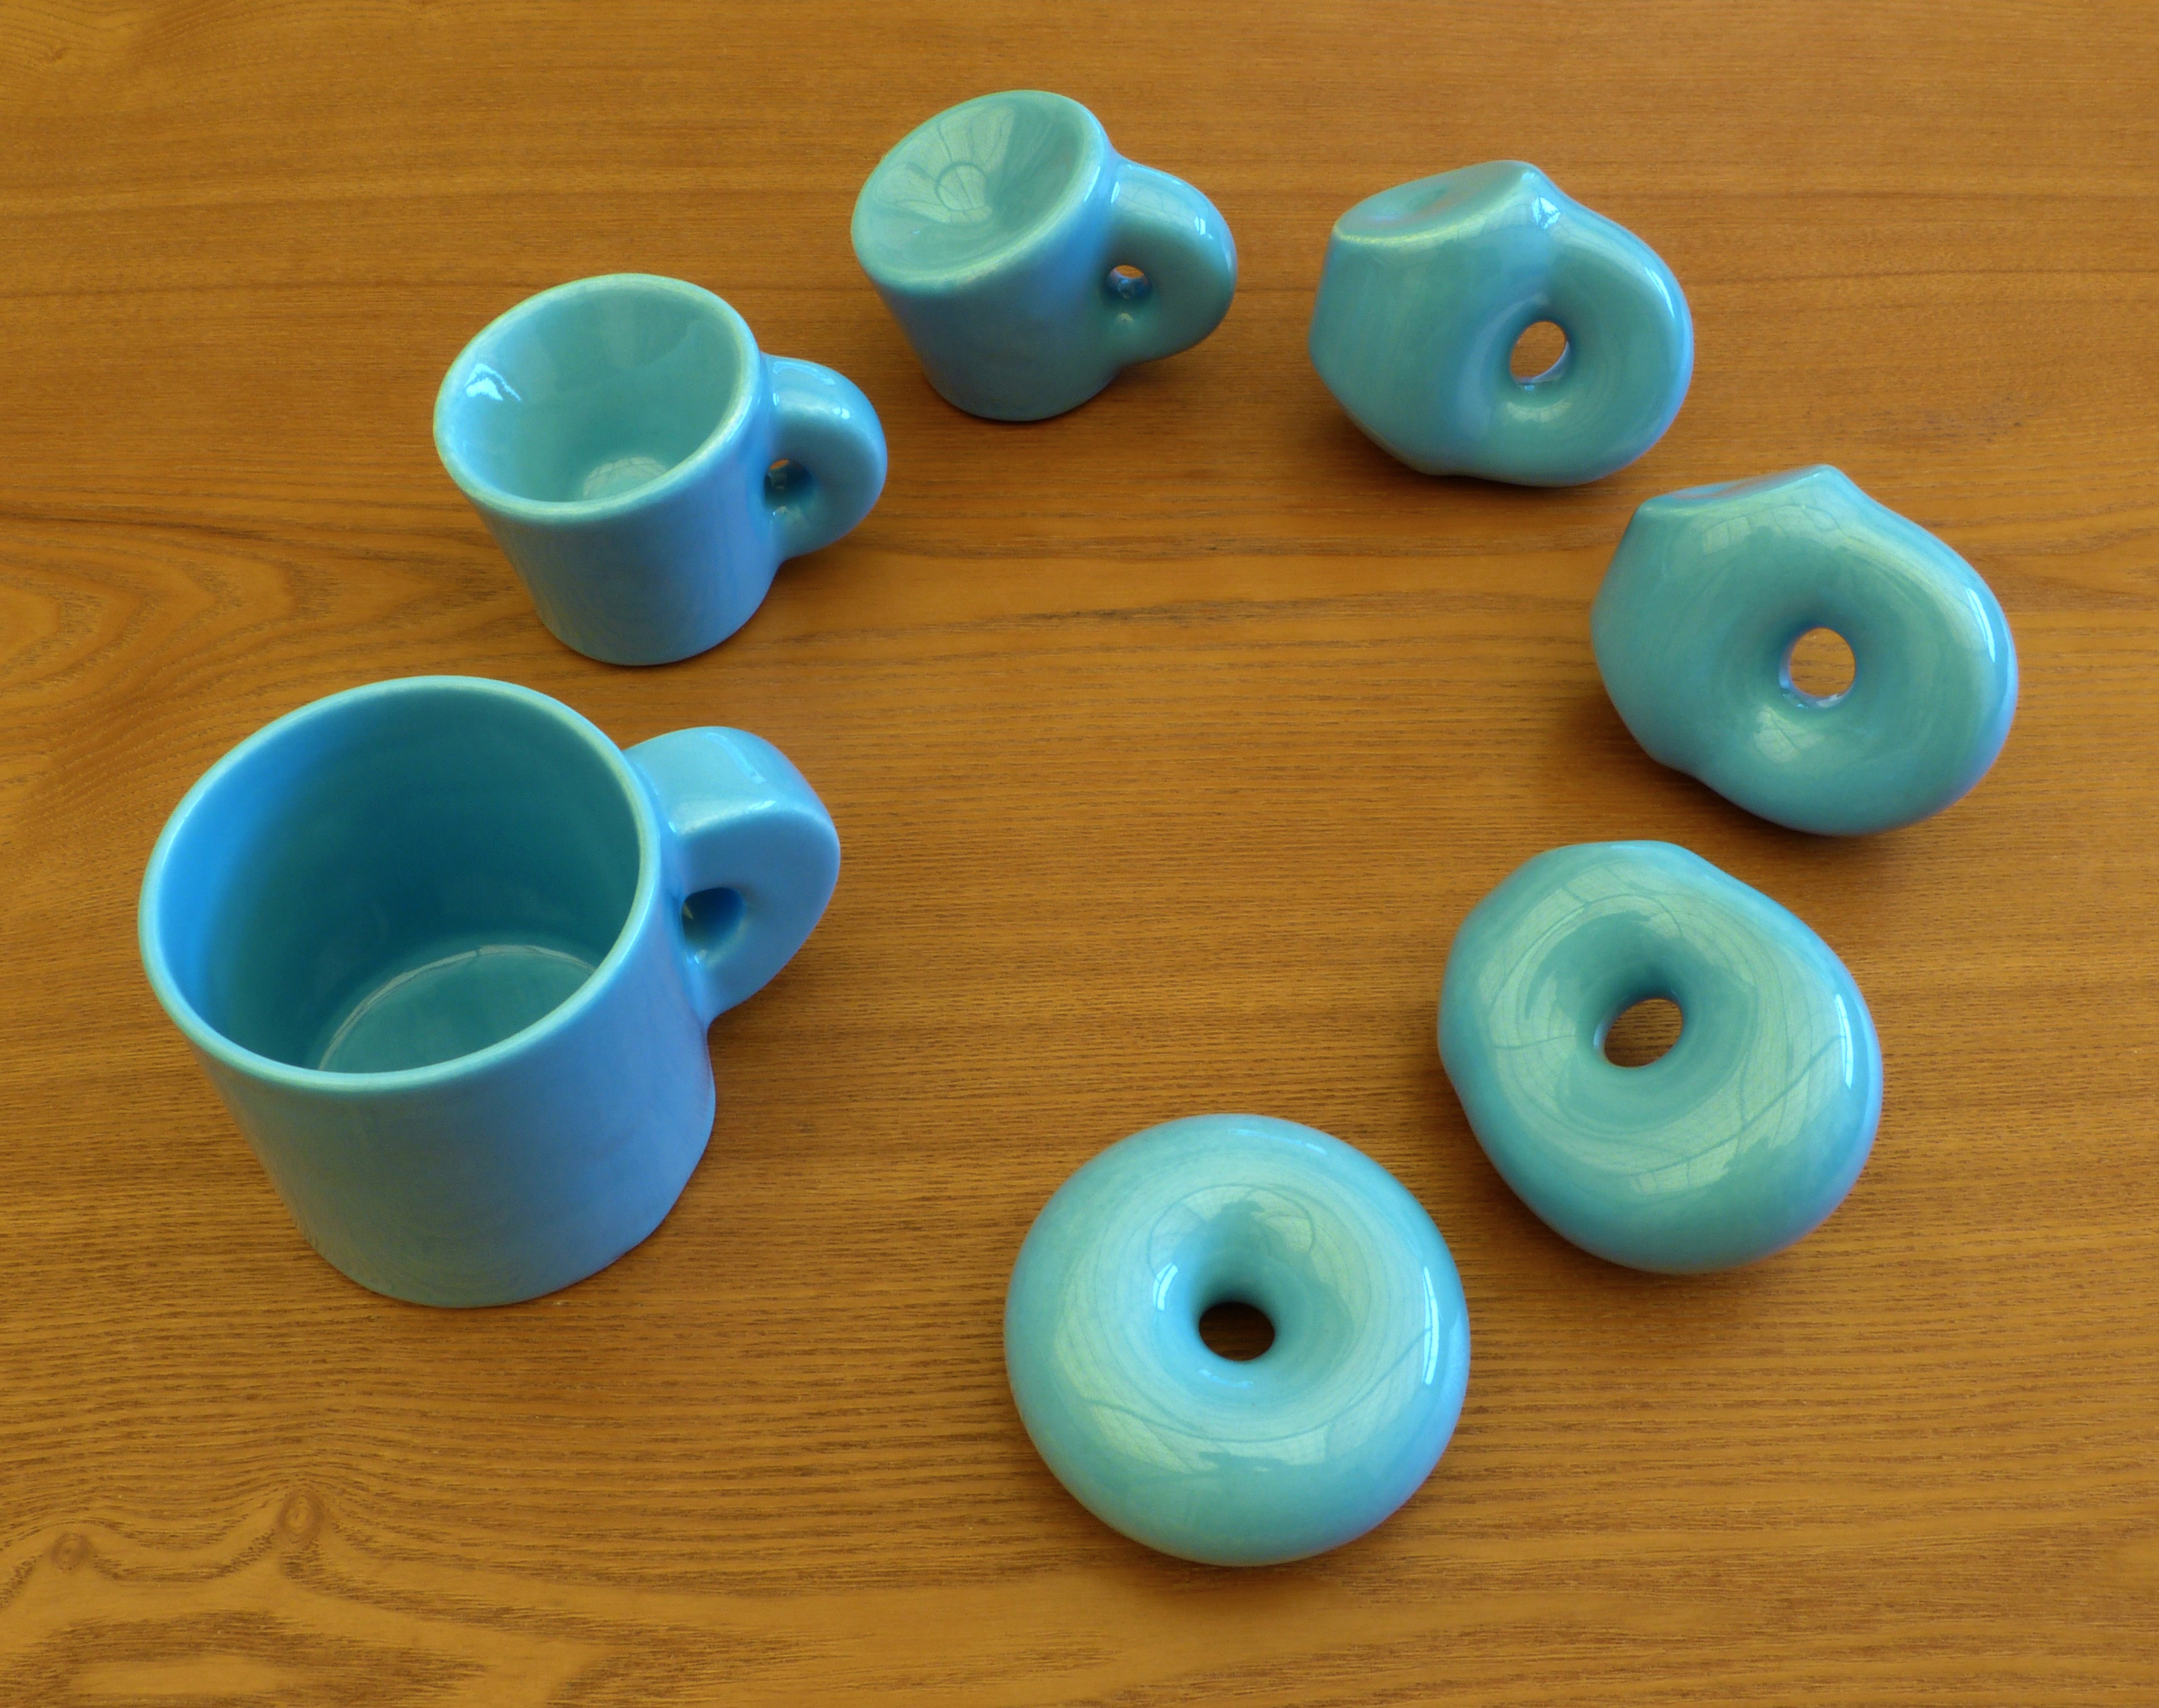
\includegraphics[scale=.035]{pics/mug-to-donut}
\end{wrapfigure}

The picture above suggests that a square and a disc have the same topology.
It might be more impressive to see that a donut is topologically equivalent to a coffee mug.
On the other hand, a disc and an annulus are topologically different.
It might be obvious, but this is a nontrivial statement
(it will follow from \ref{thm:pi1(S1)}).
So, at least not all shapes are topologically equivalent.

\begin{wrapfigure}[3]{r}{47 mm}
\vskip-4mm
\centering
\includegraphics{mppics/pic-120}
\end{wrapfigure}


\begin{thm}{Exercise}\label{ex:morning}
In the morning, a topologist looks at his clothes; there should be a T-shirt, a pair of pants, and socks.
Help him to identify each piece of clothing.
Which piece has a hole in it?

\end{thm}


\begin{thm}{Exercise}\label{ex:mug}
A topologist dropped his mug and noticed that the handle had snapped off.
``Its topology has changed,'' he thaut, ``but it can still be used for its intended purpose.''

He picked the mug up, turned it over, and said:
``Oh, I was wrong---the topology has not changed, but it is now impossible to use.''

What did he see?
\end{thm}

{

\begin{thm}{Exercise}\label{ex:finger-ring}
The topologist decided to fix the broken mug with superglue.
Being a rather clumsy person, he somehow managed to glue his index finger to his thumb---in fact, on both hands.
\begin{figure}[h!]
\centering
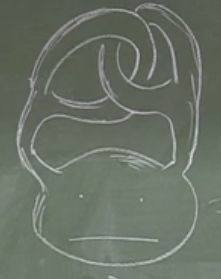
\includegraphics[scale=.3]{pics/1}
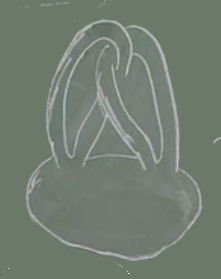
\includegraphics[scale=.3]{pics/2}
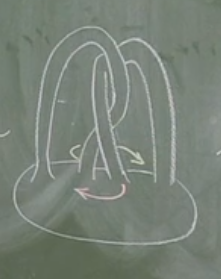
\includegraphics[scale=.3]{pics/3}
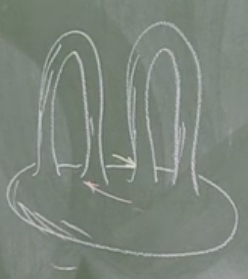
\includegraphics[scale=.3]{pics/4}
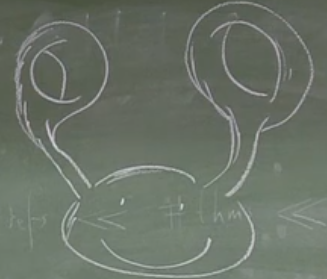
\includegraphics[scale=.3]{pics/5}
\end{figure}
Worse still, the finger rings he'd made were linked together.
But after some thinking and stretching he managed to separate the rings.

\begin{wrapfigure}{r}{19 mm}
\vskip-6mm
\centering
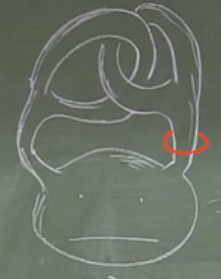
\includegraphics[scale=.3]{pics/1a}
\end{wrapfigure}

What would happen if he had a hair tie on his hand?
\end{thm}

At this point, you might think that topology has no practical value, and you are almost right, but it helps in solving the following puzzles;
these puzzles can also help you to start thinking topologically.

}

\begin{wrapfigure}{r}{25 mm}
\vskip-4mm
\centering
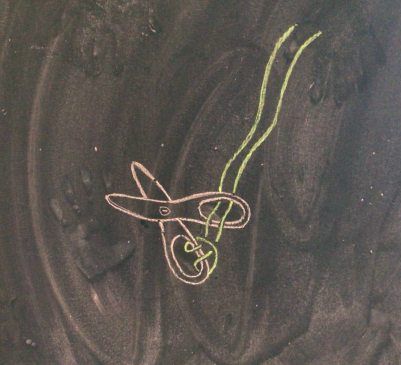
\includegraphics[scale=.2]{pics/scissors-bb}\\
\bigskip
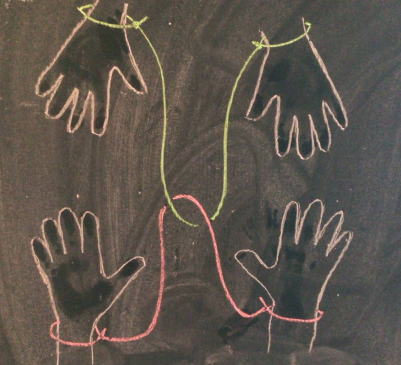
\includegraphics[scale=.2]{pics/4-hands}\\
\bigskip
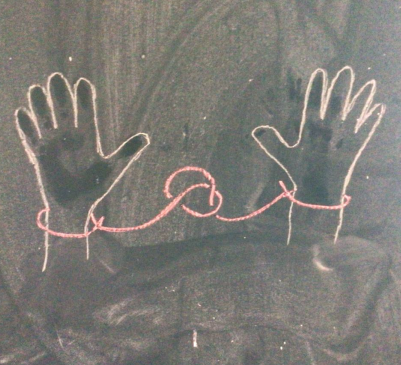
\includegraphics[scale=.2]{pics/2-hands}
\end{wrapfigure}

\begin{thm}{Exercise}\label{ex:scissors}

\begin{subthm}{ex:scissors:scissors}
Put a loop of cord thru the handles of a pair of scissors as shown.
Have someone hold the ends.
Try to get the scissors off without cutting the cord or releasing the ends.
\end{subthm}

\begin{subthm}{ex:scissors:4-hands}
Tie your hands together with a long cord;
then tie the hands of your friend in the same way, linking your cords, as shown.
Now try to get them apart without cutting the string or untying the knots.
\end{subthm}

\begin{subthm}{ex:scissors:2-hands}
If there is no friend nearby, try undoing the knot in the middle of the cord shown in the last picture.
Again, no cutting the string or untying the little knots.
\end{subthm}



\end{thm}



\include{metric}
\part{Point-set topology}
\bookmarksetupnext{startatroot,level=0}
\include{topology}
\include{sets}
\include{maps}
\include{induced}
\include{compact}
\include{metric-plus}
\include{hausdorff}
\include{connect}
%\part{Fundamental group}
%\include{path-connect}
%\include{pi1}
%\chapter{Topology meets algebra}\label{chap:algebra}

In this chapter we show that the fundamental group construction respects the maps between topological spaces\footnote{In a more fancy language, it is \index{functor}\emph{functorial}.} and behaves predictably when one changes the base point of the space.
A bit later, we will calculate the fundamental group of the circle --- this will be the first example of a space with a nontrivial fundamental group.
Once this group is calculated, the results of this chapter will lead to applications.

\section{Induced homomorphism}\label{sec:Induced homomorphism}

A \index{pointed space}\emph{pointed space} (briefly $(\c{X},x_0)$) is a topological space $\c{X}$ with a choice of base point $x_0\in \c{X}$;
so fundamental group is a construction that produces a group $\pi_1(\c{X},x_0)$ from a pointed space $(\c{X},x_0)$.

A \index{pointed map}\emph{pointed map} (briefly $f\:(\c{X},x_0)\to (\c{Y},y_0)$) is a map $f\:\c{X}\z\to \c{Y}$ with a choice of base points $x_0\in \c{X}$ and $y_0\in \c{Y}$ such that $y_0=f(x_0)$.

Let $f\:(\c{X},x_0)\to (\c{Y},y_0)$ be a continuous pointed map.
Suppose that $a_0$ and $a_1$ are loops based at $x_0$ in $\c{X}$.
Then $(f\circ a_0)$ and $(f\circ a_1)$ are loops based at $y_0$ in $\c{Y}$.
Moreover,
\[f\circ(a_0*a_1)=(f\circ a_0)*(f\circ a_1)\]
Indeed, applying the definition of the product of paths and composition of maps to $f\circ(a_0*a_1)(t)$ and $(f\circ a_0)*(f\circ a_1)(t)$ we get exactly the same expression:
\begin{align*}
\begin{cases}
f\circ a_0(2\cdot t)&\text{if}\ t\le \tfrac12,
\\
f\circ a_1(2\cdot t-1)&\text{if}\ t\ge \tfrac12.
\end{cases}
\end{align*}

Further, note that
\[a_0\sim a_1 \quad\Rightarrow\quad f\circ a_0\sim f\circ a_1.\]
Indeed, if $a_\tau$ is a homotopy from $a_0$ to $a_1$, then $f\circ a_\tau$ is a homotopy from $f\circ a_0$ to $f\circ a_1$.

It follows that the map $f\:(\c{X},x_0)\to (\c{Y},y_0)$ \index{induced homomorphism}\emph{induces} a homomorphism
\[f_*\:\pi_1(\c{X},x_0)\to \pi_1(\c{Y},y_0)\]
that is defined by $f_*\:[a]\mapsto [f\circ a]$.
(The homomorphism $f_*$ maps the homotopy class of loop $a$ to the homotopy class of loop $f\circ a$.)

Evidently, the identity map of $(\c{X},x_0)$ induces the identity homomorphism on $\pi_1(\c{X},x_0)$.
Furthermore, for any continuous pointed maps
\[(\c{X},x_0)\stackrel{f}{\to}(\c{Y},y_0)\stackrel{g}{\to}(\c{Z},z_0),\]
we have $g_*\circ f_*=(g\circ f)_*$.
These two observations will be extremely useful.

\begin{thm}{Exercise}\label{ex:retract*}
Let $A$ be a retract of $\c{X}$ with retraction $r\:\c{X}\z\to A$.
Choose $x_0\in A$; let $i\:A\to\c{X}$ be the inclusion map.
Show the following.
\begin{subthm}{ex:retract*:0}
$r_*\:\pi_1(\c{X},x_0)\to \pi_1(A,x_0)$ is a surjective homomorphism.
\end{subthm}

\begin{subthm}{ex:retract*:i}
$i_*\:\pi_1(A,x_0)\to \pi_1(\c{X},x_0)$ is an injective homomorphism.
\end{subthm}

\begin{subthm}{ex:retract*:ri}
If $A$ is a weak deformation retract, then $r_*$ and $i_*$ are isomorphisms.
\end{subthm}


\end{thm}

\section[About notation f⁎]{About notation $\bm{f_*}$}

The induced  homomorphism \index{$f_*$}$f_*\:\pi_1(\c{X},x_0)\to \pi_1(\c{Y},y_0)$ has the same direction as the original map $f\:(\c{X},x_0)\to (\c{Y},y_0)$, by that reason it is also called \index{pushforward}\emph{pushforward}.
The symbol $f_*$ (read ``$f$-star'') can be used for \textit{any} induced map of this type; for example,
one can write $f_*$ for the induced map from the set of path-connected components of $\c{X}$ to the set of path-connected components of $\c{Y}$.
The associated constructions (fundamental group or set of path-connected components) are called \index{covariant}\emph{covariant}.

If you see $f_*$, then it means it is induced by $f$, goes in the same direction and you have to guess from the context the source and target of $f_*$.

For some other constructions, the induced map might go in the opposite direction.
In this case, the induced map of $f$ is denoted by $f^*$, and called \index{pullback}\emph{pullback}.
The associated constructions are called \index{contravariant}\emph{contravariant}.

As an example of contravariant construction, consider the so-called \emph{first cohomotopy group} $\pi^1(\c{X},x_0)$, which is the set of homotopy classes of pointed continuous maps $(\c{X},x_0)\to (\SS^1,s_0)$.
(The set $\pi^1(\c{X},x_0)$ has a natural structure of abelian group, but this is not important for us.)
Then any pointed continuous map $f\:(\c{X},x_0)\to (\c{Y},y_0)$ has a pullback $f^*\:\pi^1(\c{Y},y_0)\to\pi^1(\c{X},x_0)$.
Indeed, for a map $h\:(\c{Y},y_0)\to (\SS^1,s_0)$, the composition $h\circ f$ provides a good choice of map $(\c{X},x_0)\to (\SS^1,s_0)$, so we can define $f^*[h]\df [h\circ f]$.
On the other hand, there is no good choice of map $(\c{Y},y_0)\to (\SS^1,s_0)$ for a given map $(\c{X},x_0)\to (\SS^1,s_0)$.


\section{Transport of base point}

The following theorem provides a more exact version of \ref{prop:sc=1hclass}

{

\begin{wrapfigure}[5]{r}{27 mm}
\vskip-5mm
\centering
\includegraphics{mppics/pic-1415}
\end{wrapfigure}

\begin{thm}{Theorem}
Let $c$ be a path from $x_0$ to $x_1$ in a topological space $\c{X}$.
Then $[a]\mapsto [\bar c*a*c]$ defines an isomorphism of fundamental groups $\phi_c\:\pi_1(\c{X},x_0)\to \pi_1(\c{X},x_1)$.
\end{thm}

Recall that we assume that the product of paths is taken in the usual order;
that is, \index{$a*b*c*d$} $a*b*c*d\df((a*b)*c)*d$.

}

\parit{Proof.}
Suppose $a_\tau$ is a homotopy of loops at $x_0$.
Then $\bar c*a_\tau*c$ is a homotopy of loops at $x_1$.
It follows that the map 
\[\phi_c\:[a]\mapsto [\bar c*a*c]\eqlbl{eq:[f]->[hfh]}\]
is defined.
Indeed, if $a_0\sim a_1$, then $\bar c*a_0*c\sim \bar c*a_1*c$,
which means that $[\bar c*a_0*c]=[\bar c*a_1*c]$; so the right-hand side in \ref{eq:[f]->[hfh]} does not depend on the choice of loop in the homotopy class $[a]$.

Further, if $a$ and $b$ are loops based at $x_0$, then \ref{clm:homot-claims} implies that
\begin{align*}
(\bar c*a*c)*(\bar c*b*c)&\sim \bar c*a*(c*\bar c)*b*c\sim
\\
&\sim \bar c*(a*e_{x_0})*b*c\sim
\\
&\sim \bar c*(a*b)*c.
\end{align*}
In other words,
\[\phi_c([a]\cdot [b])=\phi_c[a]\cdot \phi_c[b]\quad\text{for any}\quad [a],[b]\in \pi_1(\c{X},x_0);\]
that is, $\phi_c\:\pi_1(\c{X},x_0)\to \pi_1(\c{X},x_1)$ is a homomorphism.

The same argument shows that $\phi_{\bar c}\: \pi_1(\c{X},x_1)\to \pi_1(\c{X},x_0)$ defined by
\[\phi_{\bar c}\:[d]\mapsto [c*d*\bar c]\]
is a homomorphism.

Finally note that 
\begin{align*}
c*(\bar c*a*c)*\bar c
&\sim
(c*\bar c)*a*(c*\bar c)\sim
e_{x_0}*a*e_{x_0}\sim
a
\end{align*}
for any loop $a$ based at $x_0$.
Therefore, $\phi_{\bar c}$ is a left inverse of $\phi_c$.
The same argument shows that $\phi_{\bar c}$ is also a right inverse of $\phi_c$.
It follows that $\phi_c$ is an isomorphism.
\qeds

According to the theorem, the fundamental group%
\footnote{more precisely, its \textit{isomorphism class}}
of a path-connected space does not depend on its base point.
Therefore, for a path-connected space $\c{X}$ we do not need to specify the base point of its fundamental group.
So, if we think about the group up to isomorphism, then it is safe to write $\pi_1\c{X}$ instead of $\pi_1(\c{X},x_0)$.

\begin{thm}{Exercise}\label{ex:uphi}

\begin{subthm}{ex:uphi:uphi}
 Let $f_\tau\:\c{X}\to\c{Y}$ be a homotopy.
Consider the path defined by $c(\tau)=f_\tau(x_0)$.
Show that
\[\phi_c\circ f_{0*}=f_{1*};\]
here $f_{i*}\:\pi_1(\c{X},x_0)\to\pi_1(\c{Y},f_i(x_0))$ denotes the induced homomorphism of $f_{i}$.
\end{subthm}

\begin{subthm}{ex:uphi:hom-type}
Conclude that if two path-connected topological spaces $\c{X}$ and $\c{Y}$ have the same homotopy type, then
 their fundamental groups are isomorphic.
\end{subthm}

\end{thm}


\section{Product space}

\begin{thm}{Exercise}\label{ex:hom-product}
Let $\c{X}$ and $\c{Y}$ be two path-connected topological spaces.
Choose points $x_0\in \c{X}$ and $y_0\in \c{Y}$.
Consider the projections and their induced homomorphisms:
\begin{align*}
f\:\c{X}\times\c{Y}&\to \c{X},
&
f_*\:\pi_1(\c{X}\times\c{Y},(x_0,y_0))&\to \pi_1(\c{X},x_0),
\\
g\:\c{X}\times\c{Y}&\to \c{Y},
&
g_*\:\pi_1(\c{X}\times\c{Y},(x_0,y_0))&\to \pi_1(\c{Y},y_0).
\end{align*}
Define $\phi\:\pi_1(\c{X}\times\c{Y},(x_0,y_0))\to \pi_1(\c{X},x_0)\times \pi_1(\c{Y},y_0)$ by
\[\phi\:\alpha\mapsto (f_*(\alpha),g_*(\alpha))\]
for any $\alpha\in \pi_1(\c{X}\times\c{Y},(x_0,y_0))$.
Prove the following.

\begin{subthm}{ex:hom-product:hom}
$\phi$ is a homomorphism.
\end{subthm}


\begin{subthm}{ex:hom-product:mono}
$\phi$ is a monomorphism;
that is, if $\phi(\alpha)=\phi(\beta)$ for some $\alpha,\beta\z\in \pi_1(\c{X}\times\c{Y},(x_0,y_0))$, then
$\alpha=\beta$.
\end{subthm}

\begin{subthm}{ex:hom-product:epi}
$\phi$ is an epimorphism;
that is, for any $\gamma\in \pi_1(\c{X},x_0)\z\times\pi_1(\c{Y},y_0)$ there is $\alpha\in\pi_1(\c{X}\times\c{Y},(x_0,y_0))$ such that $\phi(\alpha)=\gamma$.
\end{subthm}

Conclude that $\pi_1(\c{X}\times\c{Y})$ is isomorphic to $\pi_1(\c{X})\times\pi_1(\c{Y})$.

\end{thm}

\begin{thm}{Advanced exercise}\label{ex:sim-product}
Let $\c{X}$ be a path-connected topological space.
Consider the quotient space $\c{Y}=(\c{X}\times \c{X})/\sim$ where $\sim$ is the minimal equivalence relation such that $(x,y)\sim (y,x)$.
Show that the fundamental group of $\c{Y}$ is commutative.
\end{thm}


%\include{homotopy}
%\include{hom-type}
%\chapter{Fundamental group of a circle}

\section{The statement}

\begin{thm}{Theorem}\label{thm:pi1(S1)}
The fundamental group of the circle $\mathbb{S}^1$ is isomorphic to the additive group of integers $\mathbb{Z}$.
\end{thm}

Given a loop $f\:[0,1]\to \mathbb{S}^1$, denote by $\deg f$ the number of times it goes aroond $\mathbb{S}^1$ counteclockwise (each clockwise turn is counded with minus).
In the following sections we will define $\deg$ formally, prove that it depends only on the homotopy class of $f$ (in other words, if $f_0\sim f_1$, then $\deg f_0=\deg f_1$) and then show that $\deg\:\pi_1(\SS^1)\to\ZZ$ is an isomorphism.

Let us show how to apply this theorem before diving into the proof.

\begin{thm}{Exercise}\label{ex:S1}
Apply the theorem to show the following.

\begin{subthm}{ex:S1:R3>R^2}
The space $\RR^3$ is not homeomorphic to the plane $\RR^2$.
\end{subthm}

\begin{subthm}{ex:D-->S}
The circle $\SS^1=\partial \DD^2$ is not a retract of the disc $\DD^2$.
\end{subthm}

\begin{subthm}{ex:bry->bry}
Given $x\in\DD^2$ the complement $\DD^2\setminus\{x\}$ is simply connected if and only if $x\in \SS^1=\partial \DD^2$.
Conclude that any homeomorphism $\DD^2\to\DD^2$ maps $\partial \DD$ to itself.
\end{subthm}

\begin{subthm}{ex:S1:finite-complement}
The complement of any finite nonempty set $F\subset\RR^2$ is not contractible.
\end{subthm}

\end{thm}

Part \ref{SHORT.ex:D-->S} in the last exercise has the following application.

\begin{thm}{Brouwer fixed point theorem in the plane}
\label{cor:brouwer-D2}
Any continuous map $f\:\DD^2\to\DD^2$ has a fixed point.
\end{thm}

\parit{Proof.}
Arguing by contradiction, assume $x\neq f(x)$ for all $x\in\DD^2$.
Consider given $x\in\DD^2$ consider the half-line $H$ from $f(x)$ to $x$.
Note that $H$ intesects $\SS^1=\partial \DD^2$ at a sinle point; denote it by $h(x)$.
Note that $h$ is continuous and $h(x)=x$ if $x\in\partial \DD^2$;
that is, $h$ defines a retruction $\DD^2\to \SS^1$.
The later contradicts \ref{ex:D-->S}.
\qeds

\begin{wrapfigure}[6]{r}{50 mm}
\vskip-6mm
\centering
\includegraphics{mppics/pic-1405}
\end{wrapfigure}

\begin{thm}{Advanced exercise}\label{ex:KK}
Consider two sets $K_1$ and $K_2$ in the plane, shown in the picture.
Each one being a closed annulus with two attached line segments.
In $K_1$ one segment is attached from the inside and another from the outside;
in $K_2$ both segments are attached from the outside.

\begin{subthm}{ex:K!=K}
Show that $K_1 \not\simeq K_2$.
\end{subthm}

\begin{subthm}{ex:K=K}
Show that $K_1 \times[0,1]\simeq K_2 \times[0,1]$.
\end{subthm}

\end{thm}


\section{Liftings}

Let us identify $\RR^2$ with the complex plane $\CC$;
namely, we will encode a point $(x,y)\in\RR^2$ by the complex number $z=x+i\cdot y$; here $i$ denotes the imaginary unit.
In particular, $\SS^1=\set{z=x+i\cdot y\in \CC}{|z|^2=x^2+y^2=1}$.

Consider the map $e\:\RR\to \mathbb{S}^1\subset \CC$ defined by
\[e\:x\mapsto \exp(2\cdot\pi\cdot i\cdot x)=\cos(2\cdot\pi\cdot x)+i\cdot\sin(2\cdot\pi\cdot x)).\]
(The last equality is called Euler's idenity, it can be taken as a definition of $\exp(2\cdot\pi\cdot i\cdot x)$.)

Let $f\:\c{X}\to \SS^1$ be a continuous map.
A continuous map $\tilde f\:\c{X}\to \RR$ will be called \index{lifting}\emph{lifting} of $f$ if $f=e\circ \tilde f$;
in other words if the following diagram \index{commutative diagram}\emph{commutes};
\begin{figure}[h!]
\centering
\begin{tikzcd}
& \RR \arrow[d, "e"]\\
\c{X} \arrow[r, "f"']\arrow[ru, "\tilde f"] & \SS^1
\end{tikzcd}
\end{figure}
the latter means that following directed paths in the diagram with the same start and endpoints lead to the same result.
Even in this simple case, using a commutative diagram is helpful, and later on you simply can't do without them.

\begin{thm}{Proposition}\label{prop:lifting}
Let $f_0\:[0,1]\to\SS^1$ be a path and let $x_0\in \RR$ be a point such that $e(x_0)=f_0(0)$.
Then there is unidue lifting $\tilde f_0$ of $f$ such that $\tilde f_0(0)=x_0$.
Moreover, if $f_0\sim f_1$ then $\tilde f_0\sim \tilde f_1$.
\end{thm}

\begin{thm}{Lemma}\label{lem:covering}
Let $W=\SS^1\setminus \{u_0\}$ for some $u_0=e(x_0)\in\SS^1$.
Then $e^{-1}(W)$ is a disjoint union of open intervals $V_n=(x_0+n,x_0+n+1)$ for $n\in \ZZ$
and $e$ defines a homeomorphism $V_n\to U$ for each $n$.

In particular, given a connected space $\c{X}$, continuous map $f\:\c{X}\z\to W$, and a point $q\in \RR$ such that $e(q)=f(p)$ for some $p\in \c{X}$ there is a unique lifting $\tilde f\:\c{X}\to \RR$ of $f$ such that $\tilde f(p)=q$.
\end{thm}


\parit{Proof.}
Observe that $e_n=e|_{V_n}$ is homeomorphism $V_n\to W$.
Indeed, $e_n$ is a continuous bijection.
Furthermore, by \ref{obs:compact-to-hausdorff} $e|_{\bar V_n}$ is a closed map.
Therefore $e_n=e|_{V_n}$ is a closed continuous bijection $V_n\to W$ and hence a homeomorphism.

Note that the intervals $V_n$ are connected components of $e^{-1}W$.
In particular, $q\in V_n$ for some $n$.
Since $\c{X}$ is connected, $\tilde f(\c{X})\subset V_n$ for any lifting $\tilde f$ lifting of $f$ such that $e(q)=f(p)$.
Since $e_n=e|_{V_n}$ is a homeomorpism, we have $\tilde f=e_n^{-1}\circ f$, which proves existance and uiqueness.
\qeds


\parit{Proof of \ref{prop:lifting}.}
Consider two open subsets $W_1=\SS^1\setminus (1,0)$ and $W_2=\SS^1\setminus (-1,0)$.
Note that $\SS^1=W_1\cup W_2$.
Therefore, $[0,1]=f^{-1}(W_1)\z\cup f^{-1}(W_2)$.

Let $\eps>0$ be the Lebesgue number of this covering; see \ref{prop:lebesgue-number}.
Consider a particition $0=t_0<t_1<\dots<t_n=1$ of $[0,1]$ into equal intervals shorter than $\eps$.
Note that $f([t_i,t_{i+1}])\subset W_1$ or  $f([t_i,t_{i+1}])\subset W_2$ for each $i$.

By \ref{lem:covering}, there is unique lifting of $f|_{[t_0,t_1]}$ such that $\tilde f(0)=x_0$; let $x_1=\tilde f(t_1)$.
By the same argument, there is unique lifting of $f|_{[t_1,t_2]}$ such that $\tilde f(t_1)=x_1$.
Repeating this argument finitely many times produces a lift of $f$, which is unique by construction.
The continuity of $f$ follows from \ref{ex:u-continuous:closed}.

\begin{wrapfigure}{r}{30 mm}
\vskip-6mm
\centering
\includegraphics{mppics/pic-1410}
\end{wrapfigure}

The proof of the last statement is similar.
Choose a homotopy $F\:[0,1]\times [0,1]\to\SS^1$ from $f_0$ to $f_1$.
Applying \ref{prop:lebesgue-number} again, we can subdivide $[0,1]\times [0,1]$ into small squares by horizontal and vertical lines so that $F$ maps each small square in $W_1$ or in $W_2$.
Then we can build the lifting $\tilde F$ square by square, from button up in the order shown in the picture.

When we extending $\tilde F$ over a small square $\square$ the value of $\tilde F$ is already defined at its lower left corner, say $v$.
So we can apply \ref{lem:covering}.
The part of $\square$ on which $\tilde F$ was already defined is one or two sides adjacent to $v$.
In both cases this set is connected and by \ref{lem:covering} the extension agrees with the already constructed part.
Again, the continuity of $\tilde F$ follows from \ref{ex:u-continuous:closed}.\qeds

\subsection*{Degree}

A loop in $\SS^1$ based at $1$ is a continuous map $f\:[0,1]\to\SS^1$
such that $f(0)=f(1)=1$.
Let $\tilde f\:[0,1]\to\RR$ be the unique lift with $\tilde f(0)=0$.
Since $e^{-1}(1)=\ZZ$, we have $\tilde f(1)\in\ZZ$.
The integer $\tilde f(1)$ will be called \index{degree of loop}\emph{degree} of the loop $f$, it will be denoted by $\deg f$.


\begin{thm}{Theorem}\label{thm:pi1S1Z}
The map $[f]\mapsto \deg f$ defines an isomorphism $\pi_1(\SS^1,1)\to\ZZ$.
\end{thm}

\parit{Proof.}
First let us show that $\deg f$ depends only on the
homotopy class of $f$.
In other words the map $[f]\mapsto \deg f$ is well defined.

Suppose $f_0$ and $f_1$ are two homotopic loops in $\SS^1$.
...

It remains to show that $\deg f_0*f_1=\deg f_0+\deg f_1$ for any two loops $f_0$ and $f_1$.
Let $\tilde f_0$ and $\tilde f_1$ be liftings of $f_0$ and $f_1$ such that $\tilde f_0(0)=\tilde f_1(0)=0$.
Recall that $\deg f_0=\tilde f_0(1)$ and $\deg f_1=\tilde f_1(1)$.
Observe that $t\mapsto \deg f_0+\tilde f_1$ is a lifting of $f_1$ s

We proved that degree defines a homomorphism $\pi_1(\SS^1,1)\cong\ZZ$;
it remains to show that this homomorphism is injective and surjective.
Surjectivity follows ???.
\qeds

\section{Fundamental theorem of algebra}

\begin{thm}{Theorem}\label{cor:FTA}
Every non-constant complex polynomial has a complex root.
\end{thm}

\parit{Proof.}
If a polynomial $p$ has no roots, then for each $r\ge 0$ the loop
$t\mapsto p(r\exp(2\pi i t))/|p(r\exp(2\pi i t))|$ lies in $\SS^1$.
For large $r$ this loop is homotopic to $t\mapsto \exp(2\pi i k t)$, where $k$ is
the degree of $p$, while for $r=0$ it is constant; this forces a change of degree,
which is impossible under a homotopy rel endpoints.


%\include{jordan}

\appendix
%\include{sol-kosniawski}

\newgeometry{top=0.9in, bottom=0.9in,inner=0.55in, outer=0.45in}
%\newgeometry{top=1.025in, bottom=1.025in,inner=0.5in, outer=0.625in, paperwidth=6.125in, paperheight=9.25in}%with bleed
{\footnotesize
\include{sols}
}



{
\newpage
\phantomsection
\footnotesize\sloppy
\documentclass[twoside]{book}
\usepackage[top=0.9in, bottom=0.9in,left=0.9in, right=0.9in, paperwidth=6in, paperheight=9in]{geometry}
\usepackage{top}

\newcommand{\spell}[2]{#1} %for text
%\newcommand{\spell}[2]{#2} %for spelling


\def\thetitle{Introduction to topology}
\def\theauthors{Anton Petrunin}

\hypersetup{
pdftitle={\thetitle}
pdfauthor={\theauthors}
}
\makeindex

%\overfullrule=100mm

\makeindex

\spell{}{\makeatletter\usepackage{environ}\RenewEnviron{figure}[1][]{ [PICTURE] }\RenewEnviron{figure*}[1][]{ [PICTURE] }\RenewEnviron{wrapfigure}[1][]{ [PICTURE] }\RenewEnviron{Figure}[1][]{ [PICTURE] }\usepackage{emptypage}\pagestyle{empty}\makeatother\usepackage[none]{hyphenat}\def\emph{\textit}\renewcommand{\footnote}[1]{\textup{\ (#1)}}\renewcommand{\frac}[2]{(#1)/(#2)}\renewcommand{\tfrac}[2]{(#1/#2)}\everydisplay{\textstyle}}

\begin{document}

%\pagestyle{empty}\def\emph{\textit}\renewcommand\includegraphics[2][{}]{}

\title{
\tt \thetitle
}
%\subtitle{\tt MATH 429, Spring 2022}
\author{\tt \theauthors}
\date{}
\maketitle
\thispagestyle{empty}

Here is very preliminary noncomplete lectures from my introductory course in topology at PennState.
They aim to be minimalist, conservative and rigourous.
I used several sources, inducing  
notes of Allen Hatcher \cite{hatcher},
lectures of Sergei Ivanov \cite{ivanov},
the textbook of Czes Kosniowski \cite{kosniowski},
and the textbook of Oleg Viro, Oleg Ivanov, Nikita Netsvetaev, and Viatcheslav Kharlamov \cite{VINKh}.

I want to thank Rostislav Matveev for his help.

Hope that someone will find it useful for something.

\medskip

\begin{flushright}
Anton Petrunin
\end{flushright}
\null\vfill\noindent{\begin{lpic}[t(-0mm),b(-0mm),r(0mm),l(0mm)]{pics/by-sa(0.5)}\end{lpic} This work is licensed under the Creative Commons Attribution-ShareAlike 4.0 International License.
To view a copy of this license, visit \texttt{http://creativecommons.org/licenses/by-sa/4.0/}}
\newpage
\cleardoublepage
\phantomsection
\pdfbookmark[0]{\contentsname}{bm:toc}
\tableofcontents

\setcounter{chapter}{-1}
\chapter{Puzzles and anecdotes}\label{chap:anecdot}



You have probably heard that for topologists, \textit{two shapes are the same if
one can be turned into the other by stretching and squeezing} (without ripping, piercing, gluing, and so on).

This statement is neither precise nor correct, but it helps build intuition.
So, imagine an object made from endlessly stretchy material that can be twisted and pulled like chewing gum;
if you can get one shape from another, then they have the same topology.
Note that the size plays no role.

\begin{figure}[!ht]
\centering
\includegraphics{mppics/pic-110}
\end{figure}

\begin{wrapfigure}{r}{47 mm}
\vskip-2mm
\centering
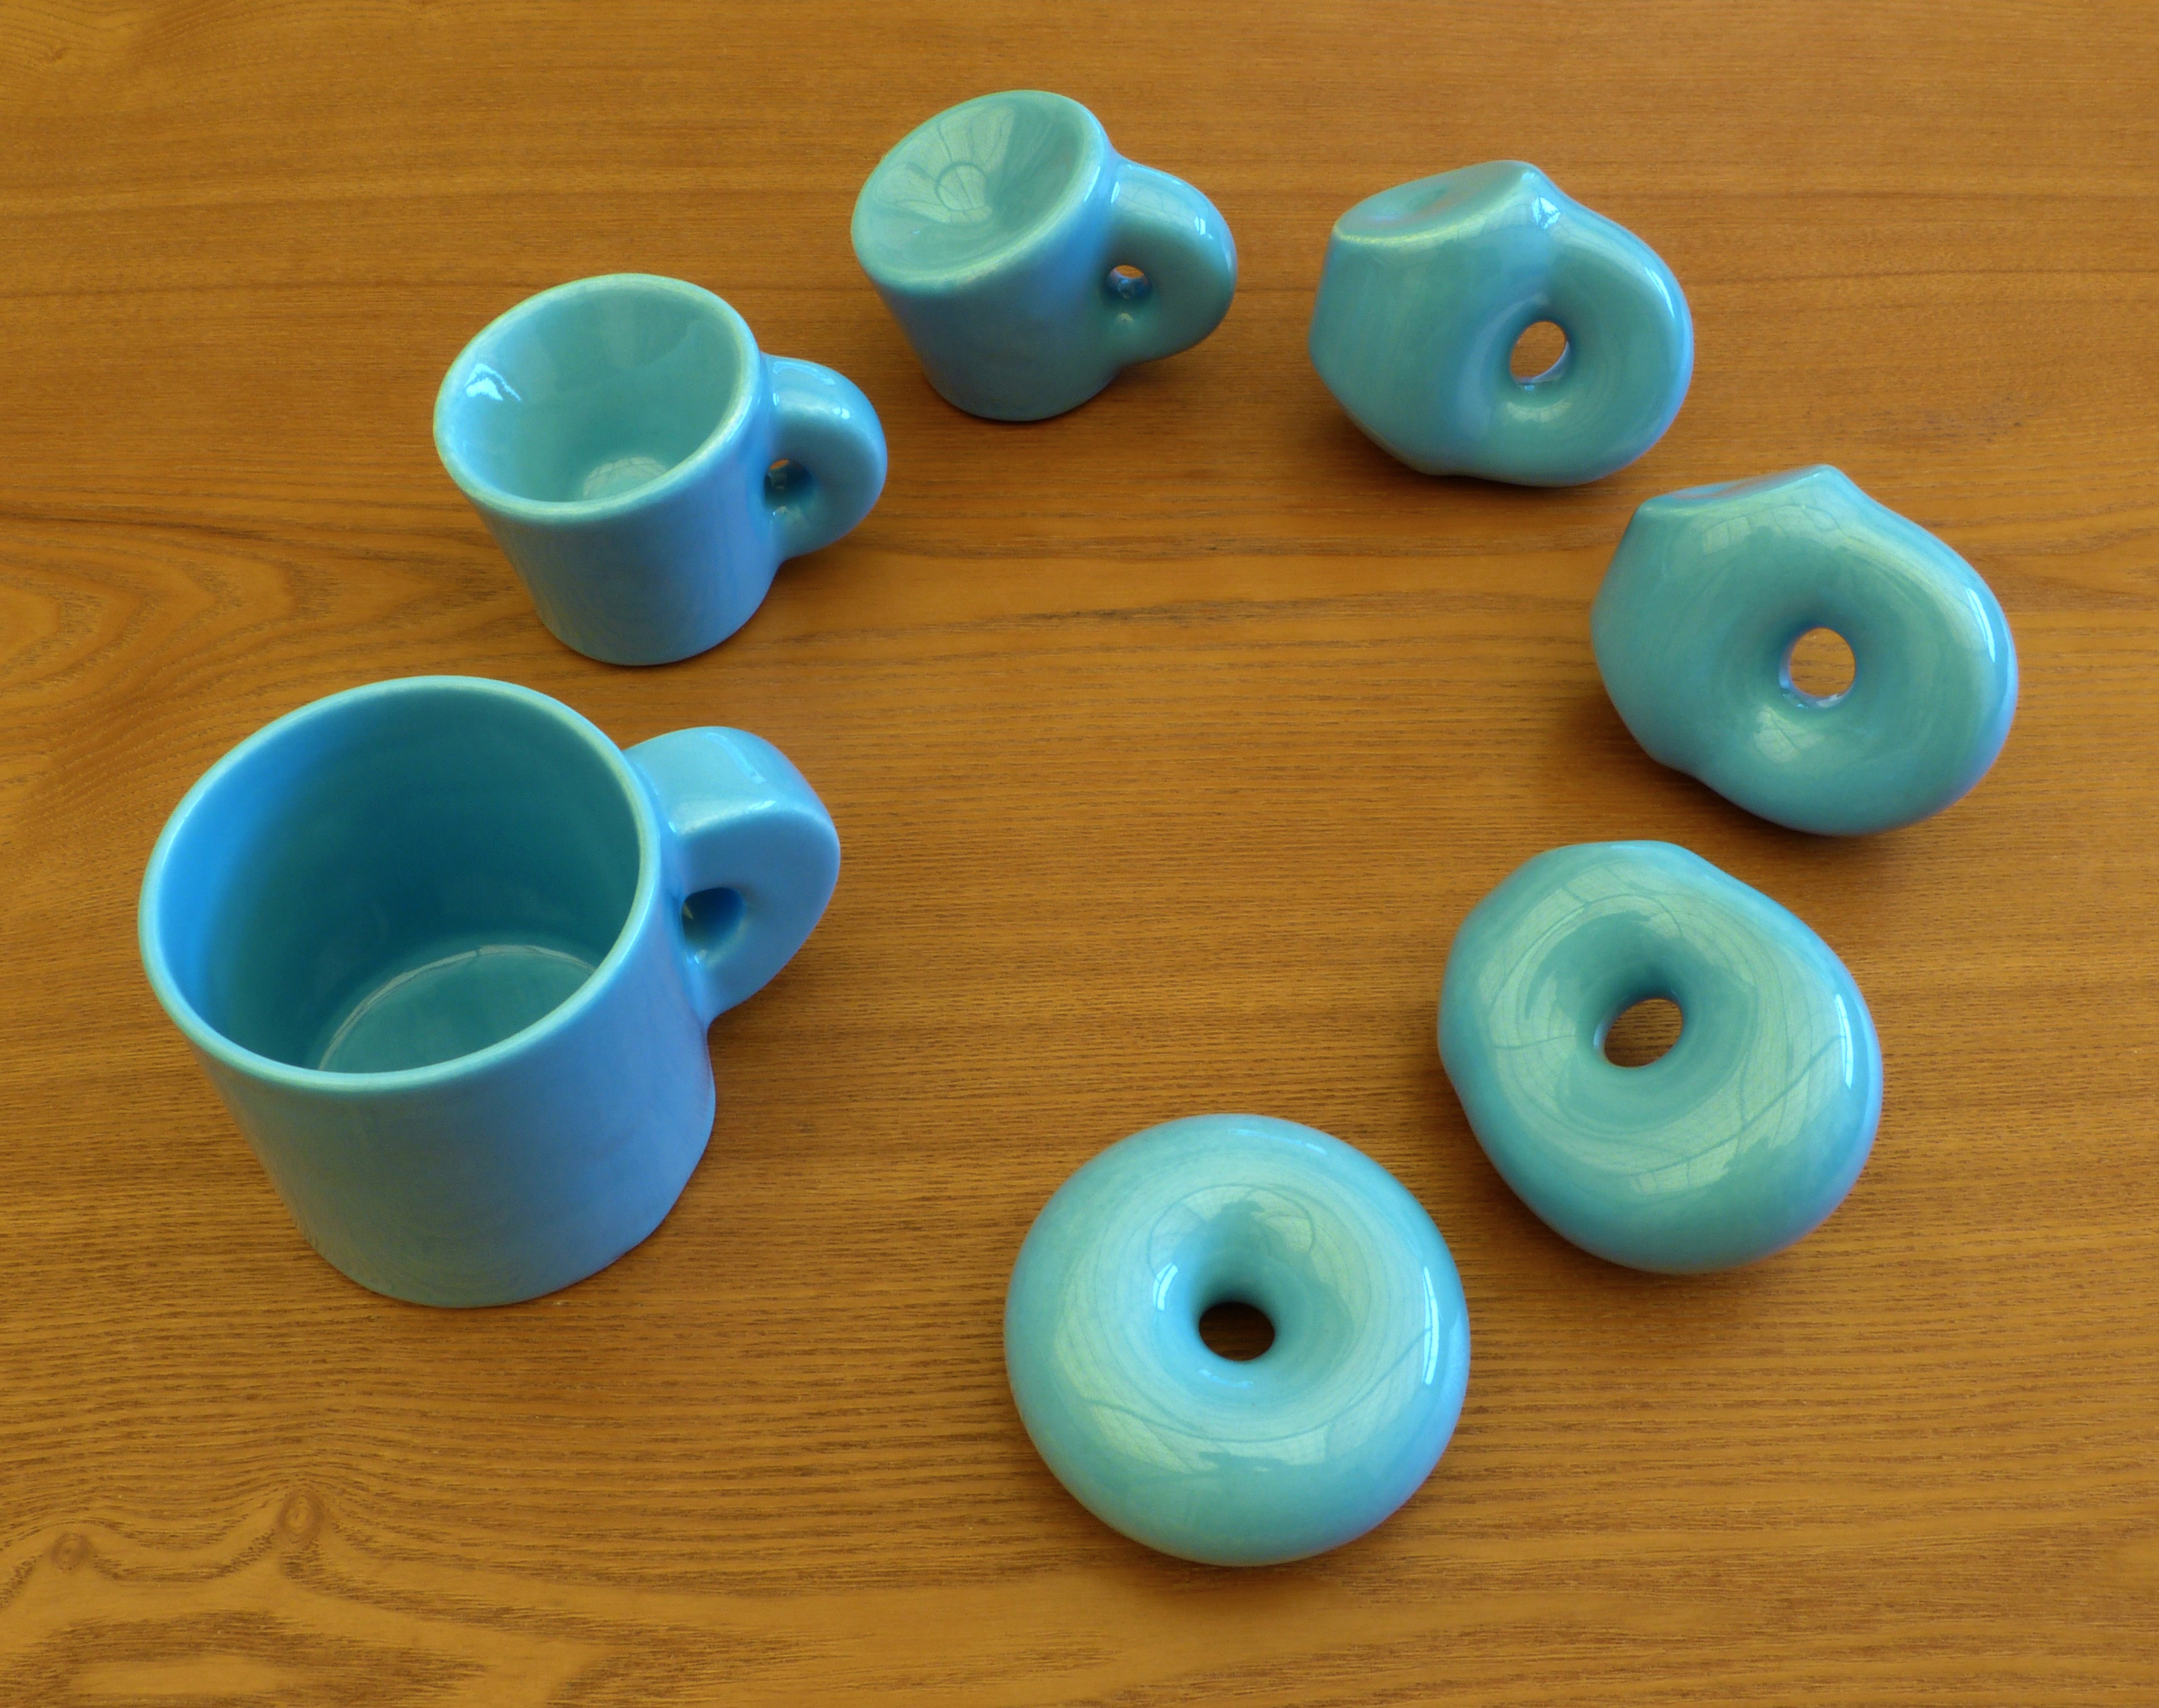
\includegraphics[scale=.035]{pics/mug-to-donut}
\end{wrapfigure}

The picture above suggests that a square and a disc have the same topology.
It might be more impressive to see that a donut is topologically equivalent to a coffee mug.
On the other hand, a disc and an annulus are topologically different.
It might be obvious, but this is a nontrivial statement
(it will follow from \ref{thm:pi1(S1)}).
So, at least not all shapes are topologically equivalent.

\begin{wrapfigure}[3]{r}{47 mm}
\vskip-4mm
\centering
\includegraphics{mppics/pic-120}
\end{wrapfigure}


\begin{thm}{Exercise}\label{ex:morning}
In the morning, a topologist looks at his clothes; there should be a T-shirt, a pair of pants, and socks.
Help him to identify each piece of clothing.
Which piece has a hole in it?

\end{thm}


\begin{thm}{Exercise}\label{ex:mug}
A topologist dropped his mug and noticed that the handle had snapped off.
``Its topology has changed,'' he thaut, ``but it can still be used for its intended purpose.''

He picked the mug up, turned it over, and said:
``Oh, I was wrong---the topology has not changed, but it is now impossible to use.''

What did he see?
\end{thm}

{

\begin{thm}{Exercise}\label{ex:finger-ring}
The topologist decided to fix the broken mug with superglue.
Being a rather clumsy person, he somehow managed to glue his index finger to his thumb---in fact, on both hands.
\begin{figure}[h!]
\centering
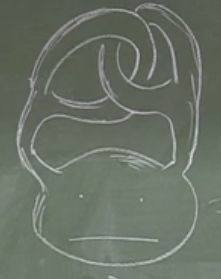
\includegraphics[scale=.3]{pics/1}
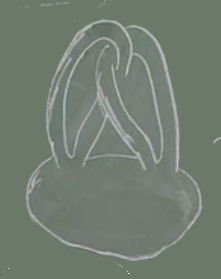
\includegraphics[scale=.3]{pics/2}
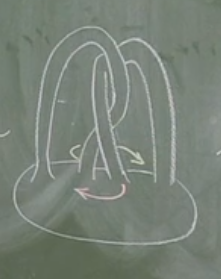
\includegraphics[scale=.3]{pics/3}
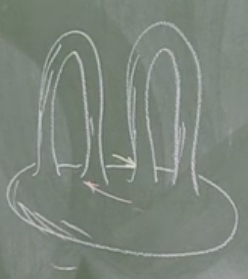
\includegraphics[scale=.3]{pics/4}
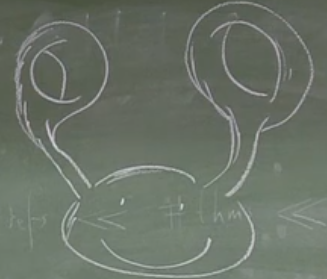
\includegraphics[scale=.3]{pics/5}
\end{figure}
Worse still, the finger rings he'd made were linked together.
But after some thinking and stretching he managed to separate the rings.

\begin{wrapfigure}{r}{19 mm}
\vskip-6mm
\centering
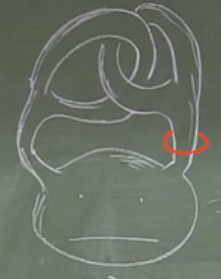
\includegraphics[scale=.3]{pics/1a}
\end{wrapfigure}

What would happen if he had a hair tie on his hand?
\end{thm}

At this point, you might think that topology has no practical value, and you are almost right, but it helps in solving the following puzzles;
these puzzles can also help you to start thinking topologically.

}

\begin{wrapfigure}{r}{25 mm}
\vskip-4mm
\centering
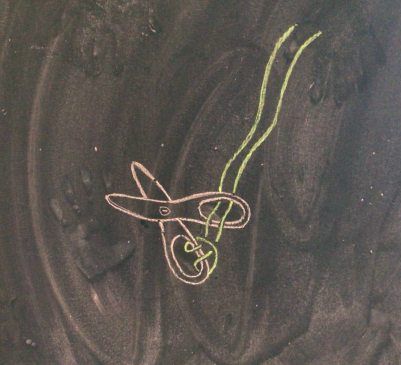
\includegraphics[scale=.2]{pics/scissors-bb}\\
\bigskip
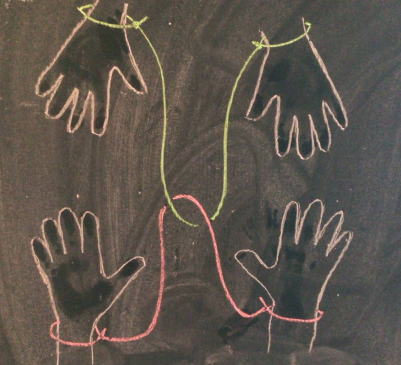
\includegraphics[scale=.2]{pics/4-hands}\\
\bigskip
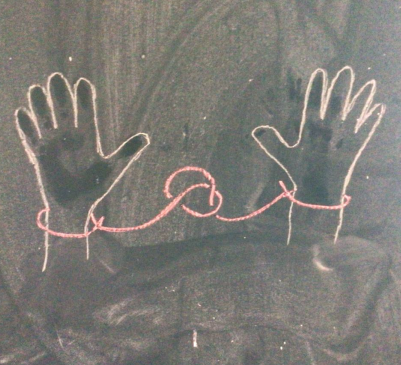
\includegraphics[scale=.2]{pics/2-hands}
\end{wrapfigure}

\begin{thm}{Exercise}\label{ex:scissors}

\begin{subthm}{ex:scissors:scissors}
Put a loop of cord thru the handles of a pair of scissors as shown.
Have someone hold the ends.
Try to get the scissors off without cutting the cord or releasing the ends.
\end{subthm}

\begin{subthm}{ex:scissors:4-hands}
Tie your hands together with a long cord;
then tie the hands of your friend in the same way, linking your cords, as shown.
Now try to get them apart without cutting the string or untying the knots.
\end{subthm}

\begin{subthm}{ex:scissors:2-hands}
If there is no friend nearby, try undoing the knot in the middle of the cord shown in the last picture.
Again, no cutting the string or untying the little knots.
\end{subthm}



\end{thm}



\include{metric}
\part{Point-set topology}
\bookmarksetupnext{startatroot,level=0}
\include{topology}
\include{sets}
\include{maps}
\include{induced}
\include{compact}
\include{metric-plus}
\include{hausdorff}
\include{connect}
%\part{Fundamental group}
%\include{path-connect}
%\include{pi1}
%\chapter{Topology meets algebra}\label{chap:algebra}

In this chapter we show that the fundamental group construction respects the maps between topological spaces\footnote{In a more fancy language, it is \index{functor}\emph{functorial}.} and behaves predictably when one changes the base point of the space.
A bit later, we will calculate the fundamental group of the circle --- this will be the first example of a space with a nontrivial fundamental group.
Once this group is calculated, the results of this chapter will lead to applications.

\section{Induced homomorphism}\label{sec:Induced homomorphism}

A \index{pointed space}\emph{pointed space} (briefly $(\c{X},x_0)$) is a topological space $\c{X}$ with a choice of base point $x_0\in \c{X}$;
so fundamental group is a construction that produces a group $\pi_1(\c{X},x_0)$ from a pointed space $(\c{X},x_0)$.

A \index{pointed map}\emph{pointed map} (briefly $f\:(\c{X},x_0)\to (\c{Y},y_0)$) is a map $f\:\c{X}\z\to \c{Y}$ with a choice of base points $x_0\in \c{X}$ and $y_0\in \c{Y}$ such that $y_0=f(x_0)$.

Let $f\:(\c{X},x_0)\to (\c{Y},y_0)$ be a continuous pointed map.
Suppose that $a_0$ and $a_1$ are loops based at $x_0$ in $\c{X}$.
Then $(f\circ a_0)$ and $(f\circ a_1)$ are loops based at $y_0$ in $\c{Y}$.
Moreover,
\[f\circ(a_0*a_1)=(f\circ a_0)*(f\circ a_1)\]
Indeed, applying the definition of the product of paths and composition of maps to $f\circ(a_0*a_1)(t)$ and $(f\circ a_0)*(f\circ a_1)(t)$ we get exactly the same expression:
\begin{align*}
\begin{cases}
f\circ a_0(2\cdot t)&\text{if}\ t\le \tfrac12,
\\
f\circ a_1(2\cdot t-1)&\text{if}\ t\ge \tfrac12.
\end{cases}
\end{align*}

Further, note that
\[a_0\sim a_1 \quad\Rightarrow\quad f\circ a_0\sim f\circ a_1.\]
Indeed, if $a_\tau$ is a homotopy from $a_0$ to $a_1$, then $f\circ a_\tau$ is a homotopy from $f\circ a_0$ to $f\circ a_1$.

It follows that the map $f\:(\c{X},x_0)\to (\c{Y},y_0)$ \index{induced homomorphism}\emph{induces} a homomorphism
\[f_*\:\pi_1(\c{X},x_0)\to \pi_1(\c{Y},y_0)\]
that is defined by $f_*\:[a]\mapsto [f\circ a]$.
(The homomorphism $f_*$ maps the homotopy class of loop $a$ to the homotopy class of loop $f\circ a$.)

Evidently, the identity map of $(\c{X},x_0)$ induces the identity homomorphism on $\pi_1(\c{X},x_0)$.
Furthermore, for any continuous pointed maps
\[(\c{X},x_0)\stackrel{f}{\to}(\c{Y},y_0)\stackrel{g}{\to}(\c{Z},z_0),\]
we have $g_*\circ f_*=(g\circ f)_*$.
These two observations will be extremely useful.

\begin{thm}{Exercise}\label{ex:retract*}
Let $A$ be a retract of $\c{X}$ with retraction $r\:\c{X}\z\to A$.
Choose $x_0\in A$; let $i\:A\to\c{X}$ be the inclusion map.
Show the following.
\begin{subthm}{ex:retract*:0}
$r_*\:\pi_1(\c{X},x_0)\to \pi_1(A,x_0)$ is a surjective homomorphism.
\end{subthm}

\begin{subthm}{ex:retract*:i}
$i_*\:\pi_1(A,x_0)\to \pi_1(\c{X},x_0)$ is an injective homomorphism.
\end{subthm}

\begin{subthm}{ex:retract*:ri}
If $A$ is a weak deformation retract, then $r_*$ and $i_*$ are isomorphisms.
\end{subthm}


\end{thm}

\section[About notation f⁎]{About notation $\bm{f_*}$}

The induced  homomorphism \index{$f_*$}$f_*\:\pi_1(\c{X},x_0)\to \pi_1(\c{Y},y_0)$ has the same direction as the original map $f\:(\c{X},x_0)\to (\c{Y},y_0)$, by that reason it is also called \index{pushforward}\emph{pushforward}.
The symbol $f_*$ (read ``$f$-star'') can be used for \textit{any} induced map of this type; for example,
one can write $f_*$ for the induced map from the set of path-connected components of $\c{X}$ to the set of path-connected components of $\c{Y}$.
The associated constructions (fundamental group or set of path-connected components) are called \index{covariant}\emph{covariant}.

If you see $f_*$, then it means it is induced by $f$, goes in the same direction and you have to guess from the context the source and target of $f_*$.

For some other constructions, the induced map might go in the opposite direction.
In this case, the induced map of $f$ is denoted by $f^*$, and called \index{pullback}\emph{pullback}.
The associated constructions are called \index{contravariant}\emph{contravariant}.

As an example of contravariant construction, consider the so-called \emph{first cohomotopy group} $\pi^1(\c{X},x_0)$, which is the set of homotopy classes of pointed continuous maps $(\c{X},x_0)\to (\SS^1,s_0)$.
(The set $\pi^1(\c{X},x_0)$ has a natural structure of abelian group, but this is not important for us.)
Then any pointed continuous map $f\:(\c{X},x_0)\to (\c{Y},y_0)$ has a pullback $f^*\:\pi^1(\c{Y},y_0)\to\pi^1(\c{X},x_0)$.
Indeed, for a map $h\:(\c{Y},y_0)\to (\SS^1,s_0)$, the composition $h\circ f$ provides a good choice of map $(\c{X},x_0)\to (\SS^1,s_0)$, so we can define $f^*[h]\df [h\circ f]$.
On the other hand, there is no good choice of map $(\c{Y},y_0)\to (\SS^1,s_0)$ for a given map $(\c{X},x_0)\to (\SS^1,s_0)$.


\section{Transport of base point}

The following theorem provides a more exact version of \ref{prop:sc=1hclass}

{

\begin{wrapfigure}[5]{r}{27 mm}
\vskip-5mm
\centering
\includegraphics{mppics/pic-1415}
\end{wrapfigure}

\begin{thm}{Theorem}
Let $c$ be a path from $x_0$ to $x_1$ in a topological space $\c{X}$.
Then $[a]\mapsto [\bar c*a*c]$ defines an isomorphism of fundamental groups $\phi_c\:\pi_1(\c{X},x_0)\to \pi_1(\c{X},x_1)$.
\end{thm}

Recall that we assume that the product of paths is taken in the usual order;
that is, \index{$a*b*c*d$} $a*b*c*d\df((a*b)*c)*d$.

}

\parit{Proof.}
Suppose $a_\tau$ is a homotopy of loops at $x_0$.
Then $\bar c*a_\tau*c$ is a homotopy of loops at $x_1$.
It follows that the map 
\[\phi_c\:[a]\mapsto [\bar c*a*c]\eqlbl{eq:[f]->[hfh]}\]
is defined.
Indeed, if $a_0\sim a_1$, then $\bar c*a_0*c\sim \bar c*a_1*c$,
which means that $[\bar c*a_0*c]=[\bar c*a_1*c]$; so the right-hand side in \ref{eq:[f]->[hfh]} does not depend on the choice of loop in the homotopy class $[a]$.

Further, if $a$ and $b$ are loops based at $x_0$, then \ref{clm:homot-claims} implies that
\begin{align*}
(\bar c*a*c)*(\bar c*b*c)&\sim \bar c*a*(c*\bar c)*b*c\sim
\\
&\sim \bar c*(a*e_{x_0})*b*c\sim
\\
&\sim \bar c*(a*b)*c.
\end{align*}
In other words,
\[\phi_c([a]\cdot [b])=\phi_c[a]\cdot \phi_c[b]\quad\text{for any}\quad [a],[b]\in \pi_1(\c{X},x_0);\]
that is, $\phi_c\:\pi_1(\c{X},x_0)\to \pi_1(\c{X},x_1)$ is a homomorphism.

The same argument shows that $\phi_{\bar c}\: \pi_1(\c{X},x_1)\to \pi_1(\c{X},x_0)$ defined by
\[\phi_{\bar c}\:[d]\mapsto [c*d*\bar c]\]
is a homomorphism.

Finally note that 
\begin{align*}
c*(\bar c*a*c)*\bar c
&\sim
(c*\bar c)*a*(c*\bar c)\sim
e_{x_0}*a*e_{x_0}\sim
a
\end{align*}
for any loop $a$ based at $x_0$.
Therefore, $\phi_{\bar c}$ is a left inverse of $\phi_c$.
The same argument shows that $\phi_{\bar c}$ is also a right inverse of $\phi_c$.
It follows that $\phi_c$ is an isomorphism.
\qeds

According to the theorem, the fundamental group%
\footnote{more precisely, its \textit{isomorphism class}}
of a path-connected space does not depend on its base point.
Therefore, for a path-connected space $\c{X}$ we do not need to specify the base point of its fundamental group.
So, if we think about the group up to isomorphism, then it is safe to write $\pi_1\c{X}$ instead of $\pi_1(\c{X},x_0)$.

\begin{thm}{Exercise}\label{ex:uphi}

\begin{subthm}{ex:uphi:uphi}
 Let $f_\tau\:\c{X}\to\c{Y}$ be a homotopy.
Consider the path defined by $c(\tau)=f_\tau(x_0)$.
Show that
\[\phi_c\circ f_{0*}=f_{1*};\]
here $f_{i*}\:\pi_1(\c{X},x_0)\to\pi_1(\c{Y},f_i(x_0))$ denotes the induced homomorphism of $f_{i}$.
\end{subthm}

\begin{subthm}{ex:uphi:hom-type}
Conclude that if two path-connected topological spaces $\c{X}$ and $\c{Y}$ have the same homotopy type, then
 their fundamental groups are isomorphic.
\end{subthm}

\end{thm}


\section{Product space}

\begin{thm}{Exercise}\label{ex:hom-product}
Let $\c{X}$ and $\c{Y}$ be two path-connected topological spaces.
Choose points $x_0\in \c{X}$ and $y_0\in \c{Y}$.
Consider the projections and their induced homomorphisms:
\begin{align*}
f\:\c{X}\times\c{Y}&\to \c{X},
&
f_*\:\pi_1(\c{X}\times\c{Y},(x_0,y_0))&\to \pi_1(\c{X},x_0),
\\
g\:\c{X}\times\c{Y}&\to \c{Y},
&
g_*\:\pi_1(\c{X}\times\c{Y},(x_0,y_0))&\to \pi_1(\c{Y},y_0).
\end{align*}
Define $\phi\:\pi_1(\c{X}\times\c{Y},(x_0,y_0))\to \pi_1(\c{X},x_0)\times \pi_1(\c{Y},y_0)$ by
\[\phi\:\alpha\mapsto (f_*(\alpha),g_*(\alpha))\]
for any $\alpha\in \pi_1(\c{X}\times\c{Y},(x_0,y_0))$.
Prove the following.

\begin{subthm}{ex:hom-product:hom}
$\phi$ is a homomorphism.
\end{subthm}


\begin{subthm}{ex:hom-product:mono}
$\phi$ is a monomorphism;
that is, if $\phi(\alpha)=\phi(\beta)$ for some $\alpha,\beta\z\in \pi_1(\c{X}\times\c{Y},(x_0,y_0))$, then
$\alpha=\beta$.
\end{subthm}

\begin{subthm}{ex:hom-product:epi}
$\phi$ is an epimorphism;
that is, for any $\gamma\in \pi_1(\c{X},x_0)\z\times\pi_1(\c{Y},y_0)$ there is $\alpha\in\pi_1(\c{X}\times\c{Y},(x_0,y_0))$ such that $\phi(\alpha)=\gamma$.
\end{subthm}

Conclude that $\pi_1(\c{X}\times\c{Y})$ is isomorphic to $\pi_1(\c{X})\times\pi_1(\c{Y})$.

\end{thm}

\begin{thm}{Advanced exercise}\label{ex:sim-product}
Let $\c{X}$ be a path-connected topological space.
Consider the quotient space $\c{Y}=(\c{X}\times \c{X})/\sim$ where $\sim$ is the minimal equivalence relation such that $(x,y)\sim (y,x)$.
Show that the fundamental group of $\c{Y}$ is commutative.
\end{thm}


%\include{homotopy}
%\include{hom-type}
%\chapter{Fundamental group of a circle}

\section{The statement}

\begin{thm}{Theorem}\label{thm:pi1(S1)}
The fundamental group of the circle $\mathbb{S}^1$ is isomorphic to the additive group of integers $\mathbb{Z}$.
\end{thm}

Given a loop $f\:[0,1]\to \mathbb{S}^1$, denote by $\deg f$ the number of times it goes aroond $\mathbb{S}^1$ counteclockwise (each clockwise turn is counded with minus).
In the following sections we will define $\deg$ formally, prove that it depends only on the homotopy class of $f$ (in other words, if $f_0\sim f_1$, then $\deg f_0=\deg f_1$) and then show that $\deg\:\pi_1(\SS^1)\to\ZZ$ is an isomorphism.

Let us show how to apply this theorem before diving into the proof.

\begin{thm}{Exercise}\label{ex:S1}
Apply the theorem to show the following.

\begin{subthm}{ex:S1:R3>R^2}
The space $\RR^3$ is not homeomorphic to the plane $\RR^2$.
\end{subthm}

\begin{subthm}{ex:D-->S}
The circle $\SS^1=\partial \DD^2$ is not a retract of the disc $\DD^2$.
\end{subthm}

\begin{subthm}{ex:bry->bry}
Given $x\in\DD^2$ the complement $\DD^2\setminus\{x\}$ is simply connected if and only if $x\in \SS^1=\partial \DD^2$.
Conclude that any homeomorphism $\DD^2\to\DD^2$ maps $\partial \DD$ to itself.
\end{subthm}

\begin{subthm}{ex:S1:finite-complement}
The complement of any finite nonempty set $F\subset\RR^2$ is not contractible.
\end{subthm}

\end{thm}

Part \ref{SHORT.ex:D-->S} in the last exercise has the following application.

\begin{thm}{Brouwer fixed point theorem in the plane}
\label{cor:brouwer-D2}
Any continuous map $f\:\DD^2\to\DD^2$ has a fixed point.
\end{thm}

\parit{Proof.}
Arguing by contradiction, assume $x\neq f(x)$ for all $x\in\DD^2$.
Consider given $x\in\DD^2$ consider the half-line $H$ from $f(x)$ to $x$.
Note that $H$ intesects $\SS^1=\partial \DD^2$ at a sinle point; denote it by $h(x)$.
Note that $h$ is continuous and $h(x)=x$ if $x\in\partial \DD^2$;
that is, $h$ defines a retruction $\DD^2\to \SS^1$.
The later contradicts \ref{ex:D-->S}.
\qeds

\begin{wrapfigure}[6]{r}{50 mm}
\vskip-6mm
\centering
\includegraphics{mppics/pic-1405}
\end{wrapfigure}

\begin{thm}{Advanced exercise}\label{ex:KK}
Consider two sets $K_1$ and $K_2$ in the plane, shown in the picture.
Each one being a closed annulus with two attached line segments.
In $K_1$ one segment is attached from the inside and another from the outside;
in $K_2$ both segments are attached from the outside.

\begin{subthm}{ex:K!=K}
Show that $K_1 \not\simeq K_2$.
\end{subthm}

\begin{subthm}{ex:K=K}
Show that $K_1 \times[0,1]\simeq K_2 \times[0,1]$.
\end{subthm}

\end{thm}


\section{Liftings}

Let us identify $\RR^2$ with the complex plane $\CC$;
namely, we will encode a point $(x,y)\in\RR^2$ by the complex number $z=x+i\cdot y$; here $i$ denotes the imaginary unit.
In particular, $\SS^1=\set{z=x+i\cdot y\in \CC}{|z|^2=x^2+y^2=1}$.

Consider the map $e\:\RR\to \mathbb{S}^1\subset \CC$ defined by
\[e\:x\mapsto \exp(2\cdot\pi\cdot i\cdot x)=\cos(2\cdot\pi\cdot x)+i\cdot\sin(2\cdot\pi\cdot x)).\]
(The last equality is called Euler's idenity, it can be taken as a definition of $\exp(2\cdot\pi\cdot i\cdot x)$.)

Let $f\:\c{X}\to \SS^1$ be a continuous map.
A continuous map $\tilde f\:\c{X}\to \RR$ will be called \index{lifting}\emph{lifting} of $f$ if $f=e\circ \tilde f$;
in other words if the following diagram \index{commutative diagram}\emph{commutes};
\begin{figure}[h!]
\centering
\begin{tikzcd}
& \RR \arrow[d, "e"]\\
\c{X} \arrow[r, "f"']\arrow[ru, "\tilde f"] & \SS^1
\end{tikzcd}
\end{figure}
the latter means that following directed paths in the diagram with the same start and endpoints lead to the same result.
Even in this simple case, using a commutative diagram is helpful, and later on you simply can't do without them.

\begin{thm}{Proposition}\label{prop:lifting}
Let $f_0\:[0,1]\to\SS^1$ be a path and let $x_0\in \RR$ be a point such that $e(x_0)=f_0(0)$.
Then there is unidue lifting $\tilde f_0$ of $f$ such that $\tilde f_0(0)=x_0$.
Moreover, if $f_0\sim f_1$ then $\tilde f_0\sim \tilde f_1$.
\end{thm}

\begin{thm}{Lemma}\label{lem:covering}
Let $W=\SS^1\setminus \{u_0\}$ for some $u_0=e(x_0)\in\SS^1$.
Then $e^{-1}(W)$ is a disjoint union of open intervals $V_n=(x_0+n,x_0+n+1)$ for $n\in \ZZ$
and $e$ defines a homeomorphism $V_n\to U$ for each $n$.

In particular, given a connected space $\c{X}$, continuous map $f\:\c{X}\z\to W$, and a point $q\in \RR$ such that $e(q)=f(p)$ for some $p\in \c{X}$ there is a unique lifting $\tilde f\:\c{X}\to \RR$ of $f$ such that $\tilde f(p)=q$.
\end{thm}


\parit{Proof.}
Observe that $e_n=e|_{V_n}$ is homeomorphism $V_n\to W$.
Indeed, $e_n$ is a continuous bijection.
Furthermore, by \ref{obs:compact-to-hausdorff} $e|_{\bar V_n}$ is a closed map.
Therefore $e_n=e|_{V_n}$ is a closed continuous bijection $V_n\to W$ and hence a homeomorphism.

Note that the intervals $V_n$ are connected components of $e^{-1}W$.
In particular, $q\in V_n$ for some $n$.
Since $\c{X}$ is connected, $\tilde f(\c{X})\subset V_n$ for any lifting $\tilde f$ lifting of $f$ such that $e(q)=f(p)$.
Since $e_n=e|_{V_n}$ is a homeomorpism, we have $\tilde f=e_n^{-1}\circ f$, which proves existance and uiqueness.
\qeds


\parit{Proof of \ref{prop:lifting}.}
Consider two open subsets $W_1=\SS^1\setminus (1,0)$ and $W_2=\SS^1\setminus (-1,0)$.
Note that $\SS^1=W_1\cup W_2$.
Therefore, $[0,1]=f^{-1}(W_1)\z\cup f^{-1}(W_2)$.

Let $\eps>0$ be the Lebesgue number of this covering; see \ref{prop:lebesgue-number}.
Consider a particition $0=t_0<t_1<\dots<t_n=1$ of $[0,1]$ into equal intervals shorter than $\eps$.
Note that $f([t_i,t_{i+1}])\subset W_1$ or  $f([t_i,t_{i+1}])\subset W_2$ for each $i$.

By \ref{lem:covering}, there is unique lifting of $f|_{[t_0,t_1]}$ such that $\tilde f(0)=x_0$; let $x_1=\tilde f(t_1)$.
By the same argument, there is unique lifting of $f|_{[t_1,t_2]}$ such that $\tilde f(t_1)=x_1$.
Repeating this argument finitely many times produces a lift of $f$, which is unique by construction.
The continuity of $f$ follows from \ref{ex:u-continuous:closed}.

\begin{wrapfigure}{r}{30 mm}
\vskip-6mm
\centering
\includegraphics{mppics/pic-1410}
\end{wrapfigure}

The proof of the last statement is similar.
Choose a homotopy $F\:[0,1]\times [0,1]\to\SS^1$ from $f_0$ to $f_1$.
Applying \ref{prop:lebesgue-number} again, we can subdivide $[0,1]\times [0,1]$ into small squares by horizontal and vertical lines so that $F$ maps each small square in $W_1$ or in $W_2$.
Then we can build the lifting $\tilde F$ square by square, from button up in the order shown in the picture.

When we extending $\tilde F$ over a small square $\square$ the value of $\tilde F$ is already defined at its lower left corner, say $v$.
So we can apply \ref{lem:covering}.
The part of $\square$ on which $\tilde F$ was already defined is one or two sides adjacent to $v$.
In both cases this set is connected and by \ref{lem:covering} the extension agrees with the already constructed part.
Again, the continuity of $\tilde F$ follows from \ref{ex:u-continuous:closed}.\qeds

\subsection*{Degree}

A loop in $\SS^1$ based at $1$ is a continuous map $f\:[0,1]\to\SS^1$
such that $f(0)=f(1)=1$.
Let $\tilde f\:[0,1]\to\RR$ be the unique lift with $\tilde f(0)=0$.
Since $e^{-1}(1)=\ZZ$, we have $\tilde f(1)\in\ZZ$.
The integer $\tilde f(1)$ will be called \index{degree of loop}\emph{degree} of the loop $f$, it will be denoted by $\deg f$.


\begin{thm}{Theorem}\label{thm:pi1S1Z}
The map $[f]\mapsto \deg f$ defines an isomorphism $\pi_1(\SS^1,1)\to\ZZ$.
\end{thm}

\parit{Proof.}
First let us show that $\deg f$ depends only on the
homotopy class of $f$.
In other words the map $[f]\mapsto \deg f$ is well defined.

Suppose $f_0$ and $f_1$ are two homotopic loops in $\SS^1$.
...

It remains to show that $\deg f_0*f_1=\deg f_0+\deg f_1$ for any two loops $f_0$ and $f_1$.
Let $\tilde f_0$ and $\tilde f_1$ be liftings of $f_0$ and $f_1$ such that $\tilde f_0(0)=\tilde f_1(0)=0$.
Recall that $\deg f_0=\tilde f_0(1)$ and $\deg f_1=\tilde f_1(1)$.
Observe that $t\mapsto \deg f_0+\tilde f_1$ is a lifting of $f_1$ s

We proved that degree defines a homomorphism $\pi_1(\SS^1,1)\cong\ZZ$;
it remains to show that this homomorphism is injective and surjective.
Surjectivity follows ???.
\qeds

\section{Fundamental theorem of algebra}

\begin{thm}{Theorem}\label{cor:FTA}
Every non-constant complex polynomial has a complex root.
\end{thm}

\parit{Proof.}
If a polynomial $p$ has no roots, then for each $r\ge 0$ the loop
$t\mapsto p(r\exp(2\pi i t))/|p(r\exp(2\pi i t))|$ lies in $\SS^1$.
For large $r$ this loop is homotopic to $t\mapsto \exp(2\pi i k t)$, where $k$ is
the degree of $p$, while for $r=0$ it is constant; this forces a change of degree,
which is impossible under a homotopy rel endpoints.


%\include{jordan}

\appendix
%\include{sol-kosniawski}

\newgeometry{top=0.9in, bottom=0.9in,inner=0.55in, outer=0.45in}
%\newgeometry{top=1.025in, bottom=1.025in,inner=0.5in, outer=0.625in, paperwidth=6.125in, paperheight=9.25in}%with bleed
{\footnotesize
\include{sols}
}



{
\newpage
\phantomsection
\footnotesize\sloppy
\documentclass[twoside]{book}
\usepackage[top=0.9in, bottom=0.9in,left=0.9in, right=0.9in, paperwidth=6in, paperheight=9in]{geometry}
\usepackage{top}

\newcommand{\spell}[2]{#1} %for text
%\newcommand{\spell}[2]{#2} %for spelling


\def\thetitle{Introduction to topology}
\def\theauthors{Anton Petrunin}

\hypersetup{
pdftitle={\thetitle}
pdfauthor={\theauthors}
}
\makeindex

%\overfullrule=100mm

\makeindex

\spell{}{\makeatletter\usepackage{environ}\RenewEnviron{figure}[1][]{ [PICTURE] }\RenewEnviron{figure*}[1][]{ [PICTURE] }\RenewEnviron{wrapfigure}[1][]{ [PICTURE] }\RenewEnviron{Figure}[1][]{ [PICTURE] }\usepackage{emptypage}\pagestyle{empty}\makeatother\usepackage[none]{hyphenat}\def\emph{\textit}\renewcommand{\footnote}[1]{\textup{\ (#1)}}\renewcommand{\frac}[2]{(#1)/(#2)}\renewcommand{\tfrac}[2]{(#1/#2)}\everydisplay{\textstyle}}

\begin{document}

%\pagestyle{empty}\def\emph{\textit}\renewcommand\includegraphics[2][{}]{}

\title{
\tt \thetitle
}
%\subtitle{\tt MATH 429, Spring 2022}
\author{\tt \theauthors}
\date{}
\maketitle
\thispagestyle{empty}

Here is very preliminary noncomplete lectures from my introductory course in topology at PennState.
They aim to be minimalist, conservative and rigourous.
I used several sources, inducing  
notes of Allen Hatcher \cite{hatcher},
lectures of Sergei Ivanov \cite{ivanov},
the textbook of Czes Kosniowski \cite{kosniowski},
and the textbook of Oleg Viro, Oleg Ivanov, Nikita Netsvetaev, and Viatcheslav Kharlamov \cite{VINKh}.

I want to thank Rostislav Matveev for his help.

Hope that someone will find it useful for something.

\medskip

\begin{flushright}
Anton Petrunin
\end{flushright}
\null\vfill\noindent{\begin{lpic}[t(-0mm),b(-0mm),r(0mm),l(0mm)]{pics/by-sa(0.5)}\end{lpic} This work is licensed under the Creative Commons Attribution-ShareAlike 4.0 International License.
To view a copy of this license, visit \texttt{http://creativecommons.org/licenses/by-sa/4.0/}}
\newpage
\cleardoublepage
\phantomsection
\pdfbookmark[0]{\contentsname}{bm:toc}
\tableofcontents

\setcounter{chapter}{-1}
\chapter{Puzzles and anecdotes}\label{chap:anecdot}



You have probably heard that for topologists, \textit{two shapes are the same if
one can be turned into the other by stretching and squeezing} (without ripping, piercing, gluing, and so on).

This statement is neither precise nor correct, but it helps build intuition.
So, imagine an object made from endlessly stretchy material that can be twisted and pulled like chewing gum;
if you can get one shape from another, then they have the same topology.
Note that the size plays no role.

\begin{figure}[!ht]
\centering
\includegraphics{mppics/pic-110}
\end{figure}

\begin{wrapfigure}{r}{47 mm}
\vskip-2mm
\centering
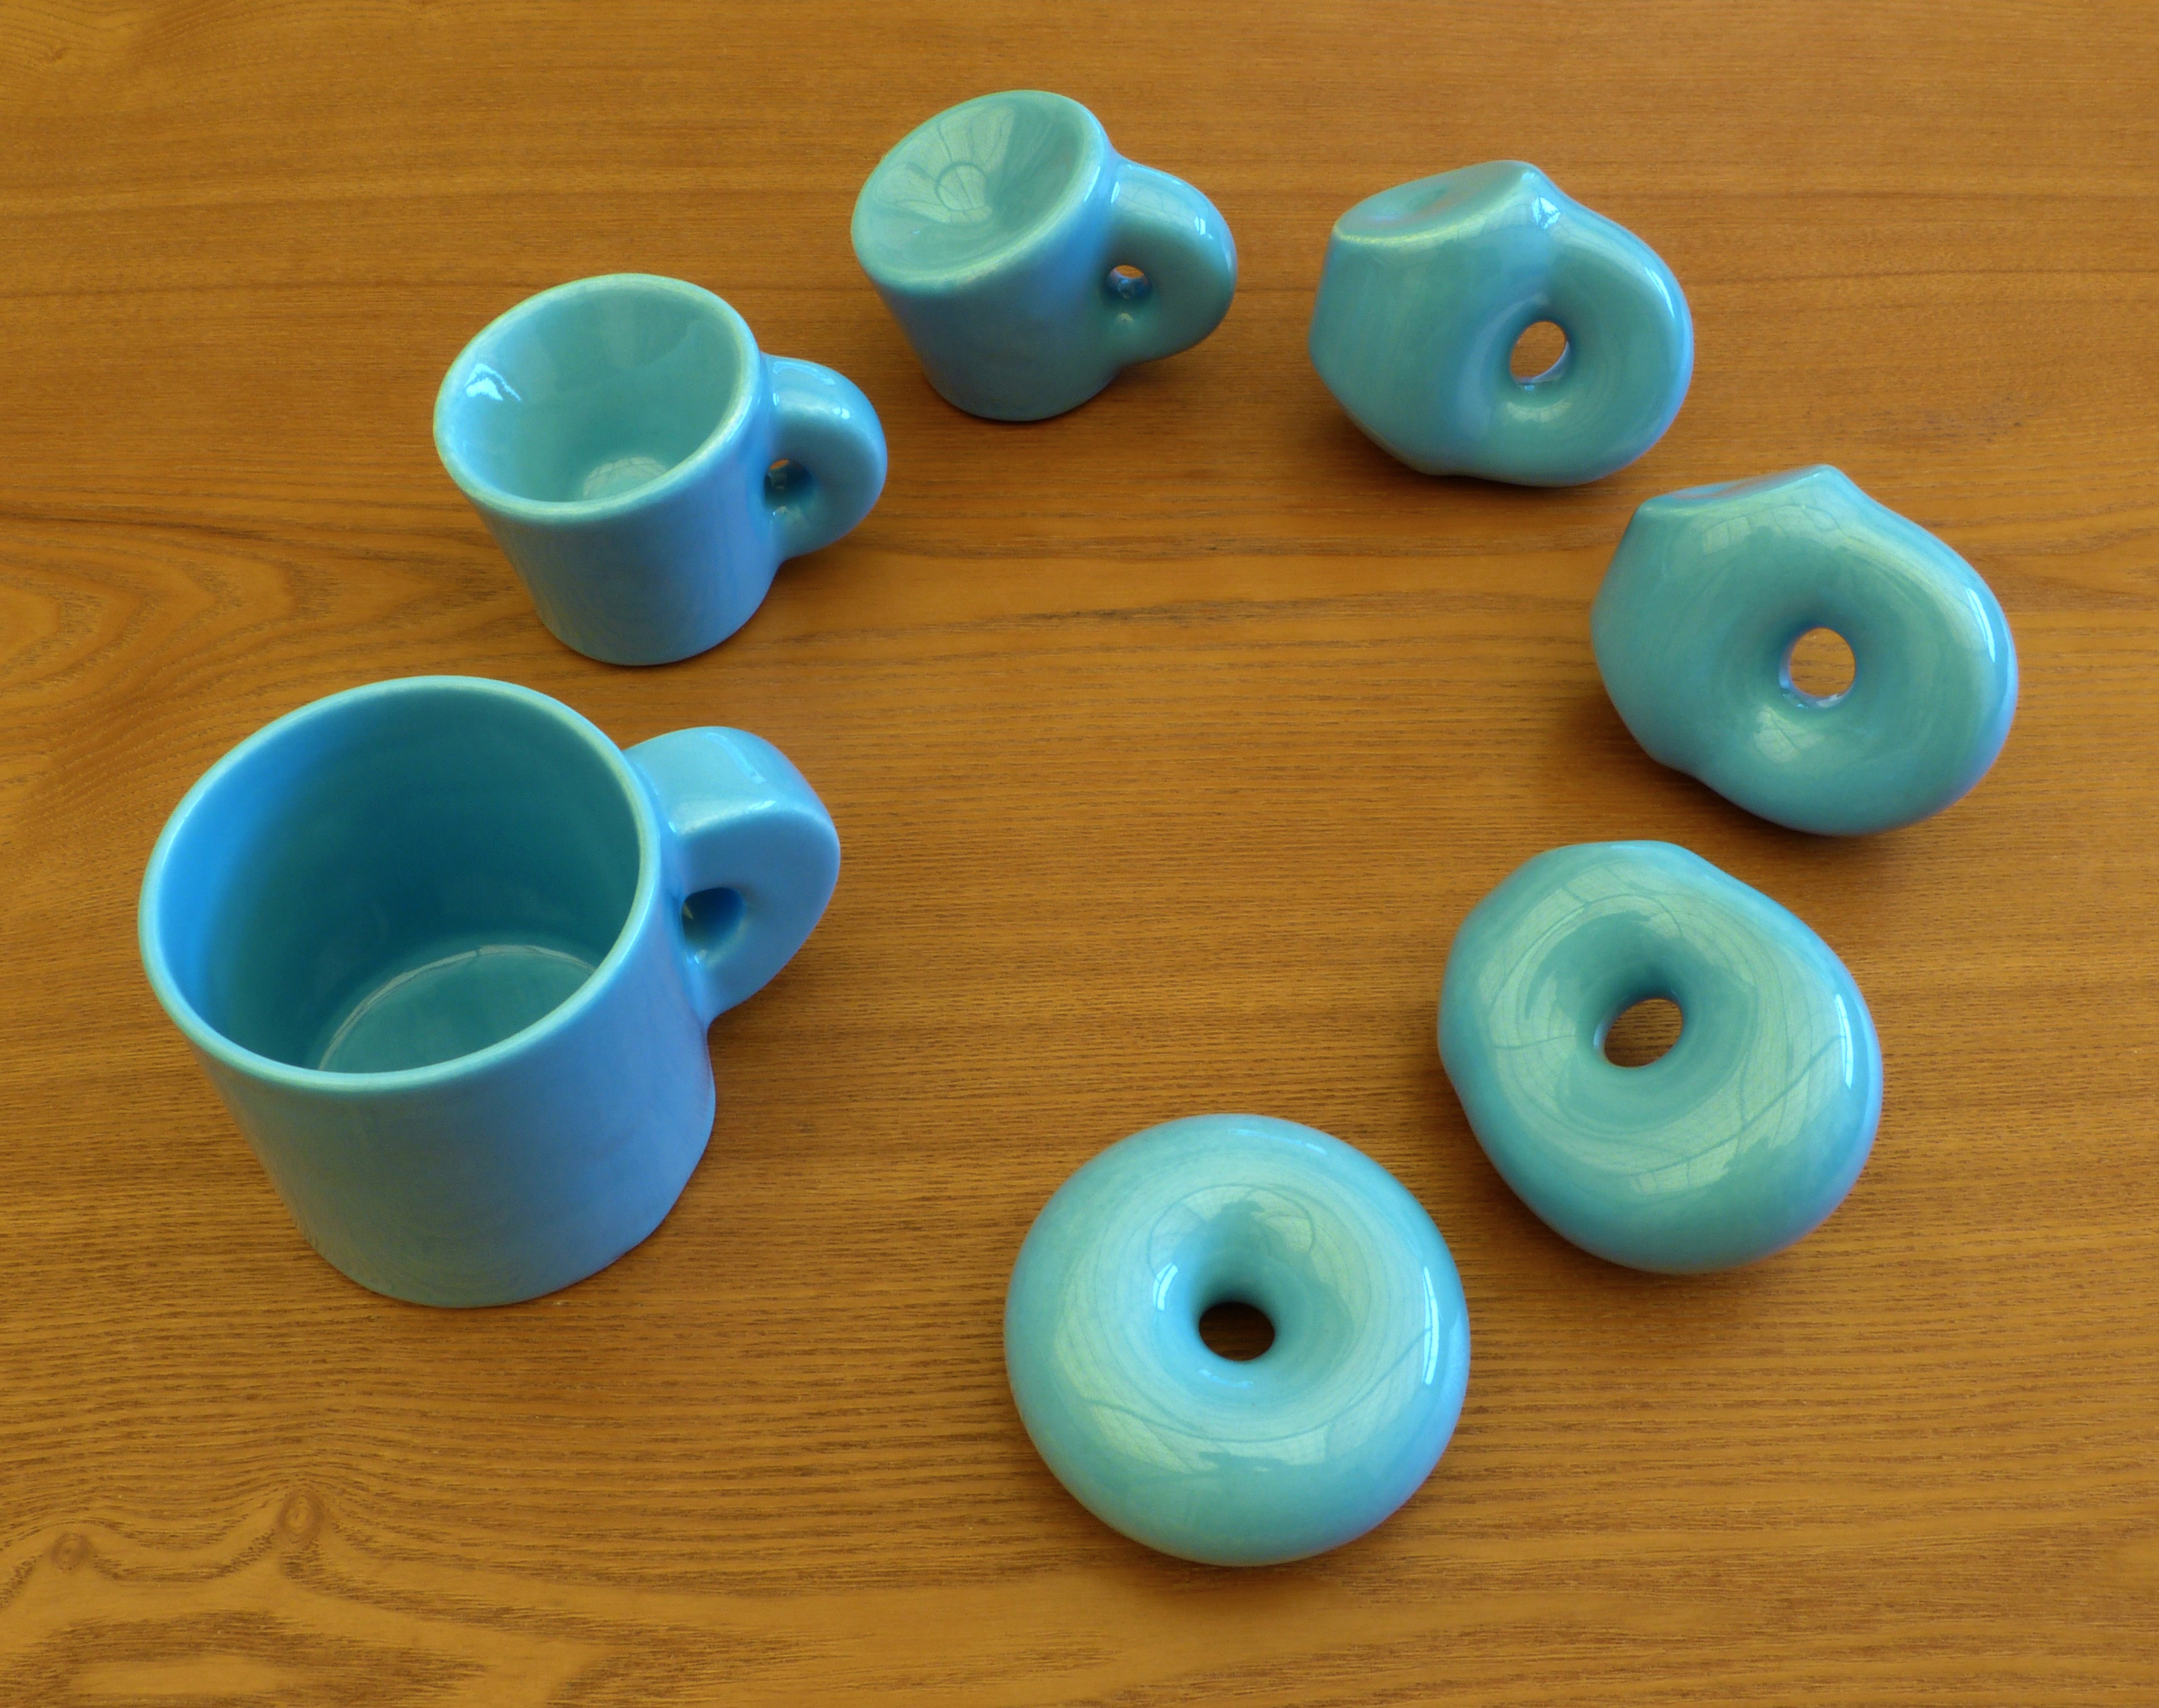
\includegraphics[scale=.035]{pics/mug-to-donut}
\end{wrapfigure}

The picture above suggests that a square and a disc have the same topology.
It might be more impressive to see that a donut is topologically equivalent to a coffee mug.
On the other hand, a disc and an annulus are topologically different.
It might be obvious, but this is a nontrivial statement
(it will follow from \ref{thm:pi1(S1)}).
So, at least not all shapes are topologically equivalent.

\begin{wrapfigure}[3]{r}{47 mm}
\vskip-4mm
\centering
\includegraphics{mppics/pic-120}
\end{wrapfigure}


\begin{thm}{Exercise}\label{ex:morning}
In the morning, a topologist looks at his clothes; there should be a T-shirt, a pair of pants, and socks.
Help him to identify each piece of clothing.
Which piece has a hole in it?

\end{thm}


\begin{thm}{Exercise}\label{ex:mug}
A topologist dropped his mug and noticed that the handle had snapped off.
``Its topology has changed,'' he thaut, ``but it can still be used for its intended purpose.''

He picked the mug up, turned it over, and said:
``Oh, I was wrong---the topology has not changed, but it is now impossible to use.''

What did he see?
\end{thm}

{

\begin{thm}{Exercise}\label{ex:finger-ring}
The topologist decided to fix the broken mug with superglue.
Being a rather clumsy person, he somehow managed to glue his index finger to his thumb---in fact, on both hands.
\begin{figure}[h!]
\centering
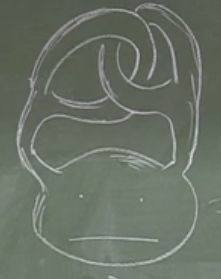
\includegraphics[scale=.3]{pics/1}
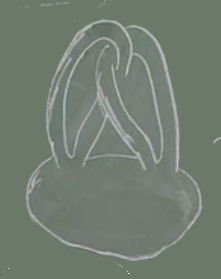
\includegraphics[scale=.3]{pics/2}
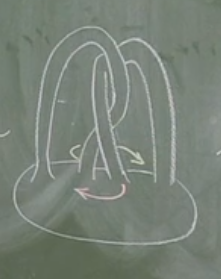
\includegraphics[scale=.3]{pics/3}
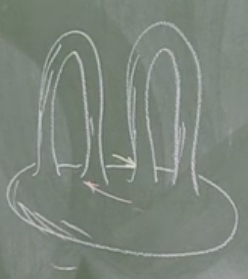
\includegraphics[scale=.3]{pics/4}
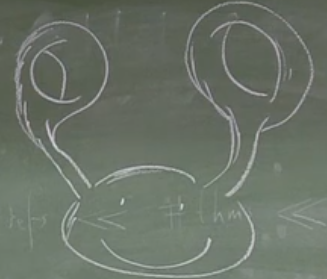
\includegraphics[scale=.3]{pics/5}
\end{figure}
Worse still, the finger rings he'd made were linked together.
But after some thinking and stretching he managed to separate the rings.

\begin{wrapfigure}{r}{19 mm}
\vskip-6mm
\centering
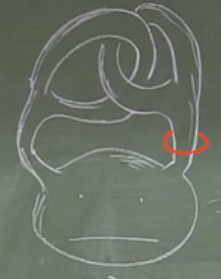
\includegraphics[scale=.3]{pics/1a}
\end{wrapfigure}

What would happen if he had a hair tie on his hand?
\end{thm}

At this point, you might think that topology has no practical value, and you are almost right, but it helps in solving the following puzzles;
these puzzles can also help you to start thinking topologically.

}

\begin{wrapfigure}{r}{25 mm}
\vskip-4mm
\centering
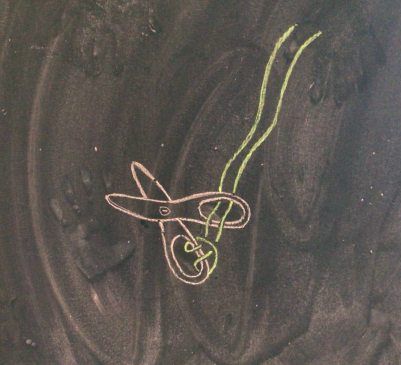
\includegraphics[scale=.2]{pics/scissors-bb}\\
\bigskip
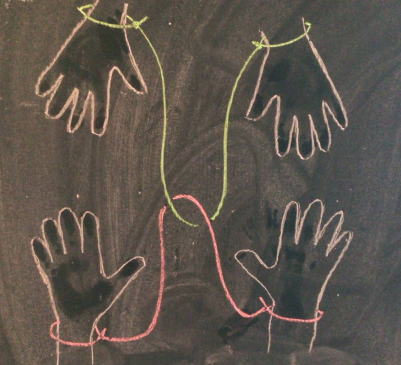
\includegraphics[scale=.2]{pics/4-hands}\\
\bigskip
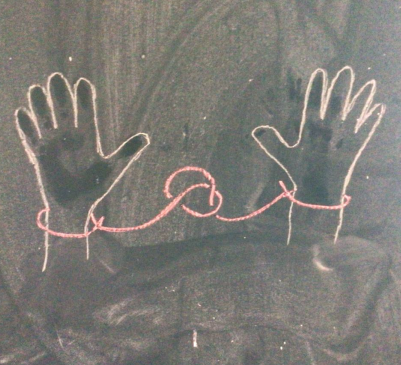
\includegraphics[scale=.2]{pics/2-hands}
\end{wrapfigure}

\begin{thm}{Exercise}\label{ex:scissors}

\begin{subthm}{ex:scissors:scissors}
Put a loop of cord thru the handles of a pair of scissors as shown.
Have someone hold the ends.
Try to get the scissors off without cutting the cord or releasing the ends.
\end{subthm}

\begin{subthm}{ex:scissors:4-hands}
Tie your hands together with a long cord;
then tie the hands of your friend in the same way, linking your cords, as shown.
Now try to get them apart without cutting the string or untying the knots.
\end{subthm}

\begin{subthm}{ex:scissors:2-hands}
If there is no friend nearby, try undoing the knot in the middle of the cord shown in the last picture.
Again, no cutting the string or untying the little knots.
\end{subthm}



\end{thm}



\include{metric}
\part{Point-set topology}
\bookmarksetupnext{startatroot,level=0}
\include{topology}
\include{sets}
\include{maps}
\include{induced}
\include{compact}
\include{metric-plus}
\include{hausdorff}
\include{connect}
%\part{Fundamental group}
%\include{path-connect}
%\include{pi1}
%\chapter{Topology meets algebra}\label{chap:algebra}

In this chapter we show that the fundamental group construction respects the maps between topological spaces\footnote{In a more fancy language, it is \index{functor}\emph{functorial}.} and behaves predictably when one changes the base point of the space.
A bit later, we will calculate the fundamental group of the circle --- this will be the first example of a space with a nontrivial fundamental group.
Once this group is calculated, the results of this chapter will lead to applications.

\section{Induced homomorphism}\label{sec:Induced homomorphism}

A \index{pointed space}\emph{pointed space} (briefly $(\c{X},x_0)$) is a topological space $\c{X}$ with a choice of base point $x_0\in \c{X}$;
so fundamental group is a construction that produces a group $\pi_1(\c{X},x_0)$ from a pointed space $(\c{X},x_0)$.

A \index{pointed map}\emph{pointed map} (briefly $f\:(\c{X},x_0)\to (\c{Y},y_0)$) is a map $f\:\c{X}\z\to \c{Y}$ with a choice of base points $x_0\in \c{X}$ and $y_0\in \c{Y}$ such that $y_0=f(x_0)$.

Let $f\:(\c{X},x_0)\to (\c{Y},y_0)$ be a continuous pointed map.
Suppose that $a_0$ and $a_1$ are loops based at $x_0$ in $\c{X}$.
Then $(f\circ a_0)$ and $(f\circ a_1)$ are loops based at $y_0$ in $\c{Y}$.
Moreover,
\[f\circ(a_0*a_1)=(f\circ a_0)*(f\circ a_1)\]
Indeed, applying the definition of the product of paths and composition of maps to $f\circ(a_0*a_1)(t)$ and $(f\circ a_0)*(f\circ a_1)(t)$ we get exactly the same expression:
\begin{align*}
\begin{cases}
f\circ a_0(2\cdot t)&\text{if}\ t\le \tfrac12,
\\
f\circ a_1(2\cdot t-1)&\text{if}\ t\ge \tfrac12.
\end{cases}
\end{align*}

Further, note that
\[a_0\sim a_1 \quad\Rightarrow\quad f\circ a_0\sim f\circ a_1.\]
Indeed, if $a_\tau$ is a homotopy from $a_0$ to $a_1$, then $f\circ a_\tau$ is a homotopy from $f\circ a_0$ to $f\circ a_1$.

It follows that the map $f\:(\c{X},x_0)\to (\c{Y},y_0)$ \index{induced homomorphism}\emph{induces} a homomorphism
\[f_*\:\pi_1(\c{X},x_0)\to \pi_1(\c{Y},y_0)\]
that is defined by $f_*\:[a]\mapsto [f\circ a]$.
(The homomorphism $f_*$ maps the homotopy class of loop $a$ to the homotopy class of loop $f\circ a$.)

Evidently, the identity map of $(\c{X},x_0)$ induces the identity homomorphism on $\pi_1(\c{X},x_0)$.
Furthermore, for any continuous pointed maps
\[(\c{X},x_0)\stackrel{f}{\to}(\c{Y},y_0)\stackrel{g}{\to}(\c{Z},z_0),\]
we have $g_*\circ f_*=(g\circ f)_*$.
These two observations will be extremely useful.

\begin{thm}{Exercise}\label{ex:retract*}
Let $A$ be a retract of $\c{X}$ with retraction $r\:\c{X}\z\to A$.
Choose $x_0\in A$; let $i\:A\to\c{X}$ be the inclusion map.
Show the following.
\begin{subthm}{ex:retract*:0}
$r_*\:\pi_1(\c{X},x_0)\to \pi_1(A,x_0)$ is a surjective homomorphism.
\end{subthm}

\begin{subthm}{ex:retract*:i}
$i_*\:\pi_1(A,x_0)\to \pi_1(\c{X},x_0)$ is an injective homomorphism.
\end{subthm}

\begin{subthm}{ex:retract*:ri}
If $A$ is a weak deformation retract, then $r_*$ and $i_*$ are isomorphisms.
\end{subthm}


\end{thm}

\section[About notation f⁎]{About notation $\bm{f_*}$}

The induced  homomorphism \index{$f_*$}$f_*\:\pi_1(\c{X},x_0)\to \pi_1(\c{Y},y_0)$ has the same direction as the original map $f\:(\c{X},x_0)\to (\c{Y},y_0)$, by that reason it is also called \index{pushforward}\emph{pushforward}.
The symbol $f_*$ (read ``$f$-star'') can be used for \textit{any} induced map of this type; for example,
one can write $f_*$ for the induced map from the set of path-connected components of $\c{X}$ to the set of path-connected components of $\c{Y}$.
The associated constructions (fundamental group or set of path-connected components) are called \index{covariant}\emph{covariant}.

If you see $f_*$, then it means it is induced by $f$, goes in the same direction and you have to guess from the context the source and target of $f_*$.

For some other constructions, the induced map might go in the opposite direction.
In this case, the induced map of $f$ is denoted by $f^*$, and called \index{pullback}\emph{pullback}.
The associated constructions are called \index{contravariant}\emph{contravariant}.

As an example of contravariant construction, consider the so-called \emph{first cohomotopy group} $\pi^1(\c{X},x_0)$, which is the set of homotopy classes of pointed continuous maps $(\c{X},x_0)\to (\SS^1,s_0)$.
(The set $\pi^1(\c{X},x_0)$ has a natural structure of abelian group, but this is not important for us.)
Then any pointed continuous map $f\:(\c{X},x_0)\to (\c{Y},y_0)$ has a pullback $f^*\:\pi^1(\c{Y},y_0)\to\pi^1(\c{X},x_0)$.
Indeed, for a map $h\:(\c{Y},y_0)\to (\SS^1,s_0)$, the composition $h\circ f$ provides a good choice of map $(\c{X},x_0)\to (\SS^1,s_0)$, so we can define $f^*[h]\df [h\circ f]$.
On the other hand, there is no good choice of map $(\c{Y},y_0)\to (\SS^1,s_0)$ for a given map $(\c{X},x_0)\to (\SS^1,s_0)$.


\section{Transport of base point}

The following theorem provides a more exact version of \ref{prop:sc=1hclass}

{

\begin{wrapfigure}[5]{r}{27 mm}
\vskip-5mm
\centering
\includegraphics{mppics/pic-1415}
\end{wrapfigure}

\begin{thm}{Theorem}
Let $c$ be a path from $x_0$ to $x_1$ in a topological space $\c{X}$.
Then $[a]\mapsto [\bar c*a*c]$ defines an isomorphism of fundamental groups $\phi_c\:\pi_1(\c{X},x_0)\to \pi_1(\c{X},x_1)$.
\end{thm}

Recall that we assume that the product of paths is taken in the usual order;
that is, \index{$a*b*c*d$} $a*b*c*d\df((a*b)*c)*d$.

}

\parit{Proof.}
Suppose $a_\tau$ is a homotopy of loops at $x_0$.
Then $\bar c*a_\tau*c$ is a homotopy of loops at $x_1$.
It follows that the map 
\[\phi_c\:[a]\mapsto [\bar c*a*c]\eqlbl{eq:[f]->[hfh]}\]
is defined.
Indeed, if $a_0\sim a_1$, then $\bar c*a_0*c\sim \bar c*a_1*c$,
which means that $[\bar c*a_0*c]=[\bar c*a_1*c]$; so the right-hand side in \ref{eq:[f]->[hfh]} does not depend on the choice of loop in the homotopy class $[a]$.

Further, if $a$ and $b$ are loops based at $x_0$, then \ref{clm:homot-claims} implies that
\begin{align*}
(\bar c*a*c)*(\bar c*b*c)&\sim \bar c*a*(c*\bar c)*b*c\sim
\\
&\sim \bar c*(a*e_{x_0})*b*c\sim
\\
&\sim \bar c*(a*b)*c.
\end{align*}
In other words,
\[\phi_c([a]\cdot [b])=\phi_c[a]\cdot \phi_c[b]\quad\text{for any}\quad [a],[b]\in \pi_1(\c{X},x_0);\]
that is, $\phi_c\:\pi_1(\c{X},x_0)\to \pi_1(\c{X},x_1)$ is a homomorphism.

The same argument shows that $\phi_{\bar c}\: \pi_1(\c{X},x_1)\to \pi_1(\c{X},x_0)$ defined by
\[\phi_{\bar c}\:[d]\mapsto [c*d*\bar c]\]
is a homomorphism.

Finally note that 
\begin{align*}
c*(\bar c*a*c)*\bar c
&\sim
(c*\bar c)*a*(c*\bar c)\sim
e_{x_0}*a*e_{x_0}\sim
a
\end{align*}
for any loop $a$ based at $x_0$.
Therefore, $\phi_{\bar c}$ is a left inverse of $\phi_c$.
The same argument shows that $\phi_{\bar c}$ is also a right inverse of $\phi_c$.
It follows that $\phi_c$ is an isomorphism.
\qeds

According to the theorem, the fundamental group%
\footnote{more precisely, its \textit{isomorphism class}}
of a path-connected space does not depend on its base point.
Therefore, for a path-connected space $\c{X}$ we do not need to specify the base point of its fundamental group.
So, if we think about the group up to isomorphism, then it is safe to write $\pi_1\c{X}$ instead of $\pi_1(\c{X},x_0)$.

\begin{thm}{Exercise}\label{ex:uphi}

\begin{subthm}{ex:uphi:uphi}
 Let $f_\tau\:\c{X}\to\c{Y}$ be a homotopy.
Consider the path defined by $c(\tau)=f_\tau(x_0)$.
Show that
\[\phi_c\circ f_{0*}=f_{1*};\]
here $f_{i*}\:\pi_1(\c{X},x_0)\to\pi_1(\c{Y},f_i(x_0))$ denotes the induced homomorphism of $f_{i}$.
\end{subthm}

\begin{subthm}{ex:uphi:hom-type}
Conclude that if two path-connected topological spaces $\c{X}$ and $\c{Y}$ have the same homotopy type, then
 their fundamental groups are isomorphic.
\end{subthm}

\end{thm}


\section{Product space}

\begin{thm}{Exercise}\label{ex:hom-product}
Let $\c{X}$ and $\c{Y}$ be two path-connected topological spaces.
Choose points $x_0\in \c{X}$ and $y_0\in \c{Y}$.
Consider the projections and their induced homomorphisms:
\begin{align*}
f\:\c{X}\times\c{Y}&\to \c{X},
&
f_*\:\pi_1(\c{X}\times\c{Y},(x_0,y_0))&\to \pi_1(\c{X},x_0),
\\
g\:\c{X}\times\c{Y}&\to \c{Y},
&
g_*\:\pi_1(\c{X}\times\c{Y},(x_0,y_0))&\to \pi_1(\c{Y},y_0).
\end{align*}
Define $\phi\:\pi_1(\c{X}\times\c{Y},(x_0,y_0))\to \pi_1(\c{X},x_0)\times \pi_1(\c{Y},y_0)$ by
\[\phi\:\alpha\mapsto (f_*(\alpha),g_*(\alpha))\]
for any $\alpha\in \pi_1(\c{X}\times\c{Y},(x_0,y_0))$.
Prove the following.

\begin{subthm}{ex:hom-product:hom}
$\phi$ is a homomorphism.
\end{subthm}


\begin{subthm}{ex:hom-product:mono}
$\phi$ is a monomorphism;
that is, if $\phi(\alpha)=\phi(\beta)$ for some $\alpha,\beta\z\in \pi_1(\c{X}\times\c{Y},(x_0,y_0))$, then
$\alpha=\beta$.
\end{subthm}

\begin{subthm}{ex:hom-product:epi}
$\phi$ is an epimorphism;
that is, for any $\gamma\in \pi_1(\c{X},x_0)\z\times\pi_1(\c{Y},y_0)$ there is $\alpha\in\pi_1(\c{X}\times\c{Y},(x_0,y_0))$ such that $\phi(\alpha)=\gamma$.
\end{subthm}

Conclude that $\pi_1(\c{X}\times\c{Y})$ is isomorphic to $\pi_1(\c{X})\times\pi_1(\c{Y})$.

\end{thm}

\begin{thm}{Advanced exercise}\label{ex:sim-product}
Let $\c{X}$ be a path-connected topological space.
Consider the quotient space $\c{Y}=(\c{X}\times \c{X})/\sim$ where $\sim$ is the minimal equivalence relation such that $(x,y)\sim (y,x)$.
Show that the fundamental group of $\c{Y}$ is commutative.
\end{thm}


%\include{homotopy}
%\include{hom-type}
%\chapter{Fundamental group of a circle}

\section{The statement}

\begin{thm}{Theorem}\label{thm:pi1(S1)}
The fundamental group of the circle $\mathbb{S}^1$ is isomorphic to the additive group of integers $\mathbb{Z}$.
\end{thm}

Given a loop $f\:[0,1]\to \mathbb{S}^1$, denote by $\deg f$ the number of times it goes aroond $\mathbb{S}^1$ counteclockwise (each clockwise turn is counded with minus).
In the following sections we will define $\deg$ formally, prove that it depends only on the homotopy class of $f$ (in other words, if $f_0\sim f_1$, then $\deg f_0=\deg f_1$) and then show that $\deg\:\pi_1(\SS^1)\to\ZZ$ is an isomorphism.

Let us show how to apply this theorem before diving into the proof.

\begin{thm}{Exercise}\label{ex:S1}
Apply the theorem to show the following.

\begin{subthm}{ex:S1:R3>R^2}
The space $\RR^3$ is not homeomorphic to the plane $\RR^2$.
\end{subthm}

\begin{subthm}{ex:D-->S}
The circle $\SS^1=\partial \DD^2$ is not a retract of the disc $\DD^2$.
\end{subthm}

\begin{subthm}{ex:bry->bry}
Given $x\in\DD^2$ the complement $\DD^2\setminus\{x\}$ is simply connected if and only if $x\in \SS^1=\partial \DD^2$.
Conclude that any homeomorphism $\DD^2\to\DD^2$ maps $\partial \DD$ to itself.
\end{subthm}

\begin{subthm}{ex:S1:finite-complement}
The complement of any finite nonempty set $F\subset\RR^2$ is not contractible.
\end{subthm}

\end{thm}

Part \ref{SHORT.ex:D-->S} in the last exercise has the following application.

\begin{thm}{Brouwer fixed point theorem in the plane}
\label{cor:brouwer-D2}
Any continuous map $f\:\DD^2\to\DD^2$ has a fixed point.
\end{thm}

\parit{Proof.}
Arguing by contradiction, assume $x\neq f(x)$ for all $x\in\DD^2$.
Consider given $x\in\DD^2$ consider the half-line $H$ from $f(x)$ to $x$.
Note that $H$ intesects $\SS^1=\partial \DD^2$ at a sinle point; denote it by $h(x)$.
Note that $h$ is continuous and $h(x)=x$ if $x\in\partial \DD^2$;
that is, $h$ defines a retruction $\DD^2\to \SS^1$.
The later contradicts \ref{ex:D-->S}.
\qeds

\begin{wrapfigure}[6]{r}{50 mm}
\vskip-6mm
\centering
\includegraphics{mppics/pic-1405}
\end{wrapfigure}

\begin{thm}{Advanced exercise}\label{ex:KK}
Consider two sets $K_1$ and $K_2$ in the plane, shown in the picture.
Each one being a closed annulus with two attached line segments.
In $K_1$ one segment is attached from the inside and another from the outside;
in $K_2$ both segments are attached from the outside.

\begin{subthm}{ex:K!=K}
Show that $K_1 \not\simeq K_2$.
\end{subthm}

\begin{subthm}{ex:K=K}
Show that $K_1 \times[0,1]\simeq K_2 \times[0,1]$.
\end{subthm}

\end{thm}


\section{Liftings}

Let us identify $\RR^2$ with the complex plane $\CC$;
namely, we will encode a point $(x,y)\in\RR^2$ by the complex number $z=x+i\cdot y$; here $i$ denotes the imaginary unit.
In particular, $\SS^1=\set{z=x+i\cdot y\in \CC}{|z|^2=x^2+y^2=1}$.

Consider the map $e\:\RR\to \mathbb{S}^1\subset \CC$ defined by
\[e\:x\mapsto \exp(2\cdot\pi\cdot i\cdot x)=\cos(2\cdot\pi\cdot x)+i\cdot\sin(2\cdot\pi\cdot x)).\]
(The last equality is called Euler's idenity, it can be taken as a definition of $\exp(2\cdot\pi\cdot i\cdot x)$.)

Let $f\:\c{X}\to \SS^1$ be a continuous map.
A continuous map $\tilde f\:\c{X}\to \RR$ will be called \index{lifting}\emph{lifting} of $f$ if $f=e\circ \tilde f$;
in other words if the following diagram \index{commutative diagram}\emph{commutes};
\begin{figure}[h!]
\centering
\begin{tikzcd}
& \RR \arrow[d, "e"]\\
\c{X} \arrow[r, "f"']\arrow[ru, "\tilde f"] & \SS^1
\end{tikzcd}
\end{figure}
the latter means that following directed paths in the diagram with the same start and endpoints lead to the same result.
Even in this simple case, using a commutative diagram is helpful, and later on you simply can't do without them.

\begin{thm}{Proposition}\label{prop:lifting}
Let $f_0\:[0,1]\to\SS^1$ be a path and let $x_0\in \RR$ be a point such that $e(x_0)=f_0(0)$.
Then there is unidue lifting $\tilde f_0$ of $f$ such that $\tilde f_0(0)=x_0$.
Moreover, if $f_0\sim f_1$ then $\tilde f_0\sim \tilde f_1$.
\end{thm}

\begin{thm}{Lemma}\label{lem:covering}
Let $W=\SS^1\setminus \{u_0\}$ for some $u_0=e(x_0)\in\SS^1$.
Then $e^{-1}(W)$ is a disjoint union of open intervals $V_n=(x_0+n,x_0+n+1)$ for $n\in \ZZ$
and $e$ defines a homeomorphism $V_n\to U$ for each $n$.

In particular, given a connected space $\c{X}$, continuous map $f\:\c{X}\z\to W$, and a point $q\in \RR$ such that $e(q)=f(p)$ for some $p\in \c{X}$ there is a unique lifting $\tilde f\:\c{X}\to \RR$ of $f$ such that $\tilde f(p)=q$.
\end{thm}


\parit{Proof.}
Observe that $e_n=e|_{V_n}$ is homeomorphism $V_n\to W$.
Indeed, $e_n$ is a continuous bijection.
Furthermore, by \ref{obs:compact-to-hausdorff} $e|_{\bar V_n}$ is a closed map.
Therefore $e_n=e|_{V_n}$ is a closed continuous bijection $V_n\to W$ and hence a homeomorphism.

Note that the intervals $V_n$ are connected components of $e^{-1}W$.
In particular, $q\in V_n$ for some $n$.
Since $\c{X}$ is connected, $\tilde f(\c{X})\subset V_n$ for any lifting $\tilde f$ lifting of $f$ such that $e(q)=f(p)$.
Since $e_n=e|_{V_n}$ is a homeomorpism, we have $\tilde f=e_n^{-1}\circ f$, which proves existance and uiqueness.
\qeds


\parit{Proof of \ref{prop:lifting}.}
Consider two open subsets $W_1=\SS^1\setminus (1,0)$ and $W_2=\SS^1\setminus (-1,0)$.
Note that $\SS^1=W_1\cup W_2$.
Therefore, $[0,1]=f^{-1}(W_1)\z\cup f^{-1}(W_2)$.

Let $\eps>0$ be the Lebesgue number of this covering; see \ref{prop:lebesgue-number}.
Consider a particition $0=t_0<t_1<\dots<t_n=1$ of $[0,1]$ into equal intervals shorter than $\eps$.
Note that $f([t_i,t_{i+1}])\subset W_1$ or  $f([t_i,t_{i+1}])\subset W_2$ for each $i$.

By \ref{lem:covering}, there is unique lifting of $f|_{[t_0,t_1]}$ such that $\tilde f(0)=x_0$; let $x_1=\tilde f(t_1)$.
By the same argument, there is unique lifting of $f|_{[t_1,t_2]}$ such that $\tilde f(t_1)=x_1$.
Repeating this argument finitely many times produces a lift of $f$, which is unique by construction.
The continuity of $f$ follows from \ref{ex:u-continuous:closed}.

\begin{wrapfigure}{r}{30 mm}
\vskip-6mm
\centering
\includegraphics{mppics/pic-1410}
\end{wrapfigure}

The proof of the last statement is similar.
Choose a homotopy $F\:[0,1]\times [0,1]\to\SS^1$ from $f_0$ to $f_1$.
Applying \ref{prop:lebesgue-number} again, we can subdivide $[0,1]\times [0,1]$ into small squares by horizontal and vertical lines so that $F$ maps each small square in $W_1$ or in $W_2$.
Then we can build the lifting $\tilde F$ square by square, from button up in the order shown in the picture.

When we extending $\tilde F$ over a small square $\square$ the value of $\tilde F$ is already defined at its lower left corner, say $v$.
So we can apply \ref{lem:covering}.
The part of $\square$ on which $\tilde F$ was already defined is one or two sides adjacent to $v$.
In both cases this set is connected and by \ref{lem:covering} the extension agrees with the already constructed part.
Again, the continuity of $\tilde F$ follows from \ref{ex:u-continuous:closed}.\qeds

\subsection*{Degree}

A loop in $\SS^1$ based at $1$ is a continuous map $f\:[0,1]\to\SS^1$
such that $f(0)=f(1)=1$.
Let $\tilde f\:[0,1]\to\RR$ be the unique lift with $\tilde f(0)=0$.
Since $e^{-1}(1)=\ZZ$, we have $\tilde f(1)\in\ZZ$.
The integer $\tilde f(1)$ will be called \index{degree of loop}\emph{degree} of the loop $f$, it will be denoted by $\deg f$.


\begin{thm}{Theorem}\label{thm:pi1S1Z}
The map $[f]\mapsto \deg f$ defines an isomorphism $\pi_1(\SS^1,1)\to\ZZ$.
\end{thm}

\parit{Proof.}
First let us show that $\deg f$ depends only on the
homotopy class of $f$.
In other words the map $[f]\mapsto \deg f$ is well defined.

Suppose $f_0$ and $f_1$ are two homotopic loops in $\SS^1$.
...

It remains to show that $\deg f_0*f_1=\deg f_0+\deg f_1$ for any two loops $f_0$ and $f_1$.
Let $\tilde f_0$ and $\tilde f_1$ be liftings of $f_0$ and $f_1$ such that $\tilde f_0(0)=\tilde f_1(0)=0$.
Recall that $\deg f_0=\tilde f_0(1)$ and $\deg f_1=\tilde f_1(1)$.
Observe that $t\mapsto \deg f_0+\tilde f_1$ is a lifting of $f_1$ s

We proved that degree defines a homomorphism $\pi_1(\SS^1,1)\cong\ZZ$;
it remains to show that this homomorphism is injective and surjective.
Surjectivity follows ???.
\qeds

\section{Fundamental theorem of algebra}

\begin{thm}{Theorem}\label{cor:FTA}
Every non-constant complex polynomial has a complex root.
\end{thm}

\parit{Proof.}
If a polynomial $p$ has no roots, then for each $r\ge 0$ the loop
$t\mapsto p(r\exp(2\pi i t))/|p(r\exp(2\pi i t))|$ lies in $\SS^1$.
For large $r$ this loop is homotopic to $t\mapsto \exp(2\pi i k t)$, where $k$ is
the degree of $p$, while for $r=0$ it is constant; this forces a change of degree,
which is impossible under a homotopy rel endpoints.


%\include{jordan}

\appendix
%\include{sol-kosniawski}

\newgeometry{top=0.9in, bottom=0.9in,inner=0.55in, outer=0.45in}
%\newgeometry{top=1.025in, bottom=1.025in,inner=0.5in, outer=0.625in, paperwidth=6.125in, paperheight=9.25in}%with bleed
{\footnotesize
\include{sols}
}



{
\newpage
\phantomsection
\footnotesize\sloppy
\documentclass[twoside]{book}
\usepackage[top=0.9in, bottom=0.9in,left=0.9in, right=0.9in, paperwidth=6in, paperheight=9in]{geometry}
\usepackage{top}

\newcommand{\spell}[2]{#1} %for text
%\newcommand{\spell}[2]{#2} %for spelling


\def\thetitle{Introduction to topology}
\def\theauthors{Anton Petrunin}

\hypersetup{
pdftitle={\thetitle}
pdfauthor={\theauthors}
}
\makeindex

%\overfullrule=100mm

\makeindex

\spell{}{\makeatletter\usepackage{environ}\RenewEnviron{figure}[1][]{ [PICTURE] }\RenewEnviron{figure*}[1][]{ [PICTURE] }\RenewEnviron{wrapfigure}[1][]{ [PICTURE] }\RenewEnviron{Figure}[1][]{ [PICTURE] }\usepackage{emptypage}\pagestyle{empty}\makeatother\usepackage[none]{hyphenat}\def\emph{\textit}\renewcommand{\footnote}[1]{\textup{\ (#1)}}\renewcommand{\frac}[2]{(#1)/(#2)}\renewcommand{\tfrac}[2]{(#1/#2)}\everydisplay{\textstyle}}

\begin{document}

%\pagestyle{empty}\def\emph{\textit}\renewcommand\includegraphics[2][{}]{}

\title{
\tt \thetitle
}
%\subtitle{\tt MATH 429, Spring 2022}
\author{\tt \theauthors}
\date{}
\maketitle
\thispagestyle{empty}

Here is very preliminary noncomplete lectures from my introductory course in topology at PennState.
They aim to be minimalist, conservative and rigourous.
I used several sources, inducing  
notes of Allen Hatcher \cite{hatcher},
lectures of Sergei Ivanov \cite{ivanov},
the textbook of Czes Kosniowski \cite{kosniowski},
and the textbook of Oleg Viro, Oleg Ivanov, Nikita Netsvetaev, and Viatcheslav Kharlamov \cite{VINKh}.

I want to thank Rostislav Matveev for his help.

Hope that someone will find it useful for something.

\medskip

\begin{flushright}
Anton Petrunin
\end{flushright}
\null\vfill\noindent{\begin{lpic}[t(-0mm),b(-0mm),r(0mm),l(0mm)]{pics/by-sa(0.5)}\end{lpic} This work is licensed under the Creative Commons Attribution-ShareAlike 4.0 International License.
To view a copy of this license, visit \texttt{http://creativecommons.org/licenses/by-sa/4.0/}}
\newpage
\cleardoublepage
\phantomsection
\pdfbookmark[0]{\contentsname}{bm:toc}
\tableofcontents

\include{anekdot}
\include{metric}
\part{Point-set topology}
\bookmarksetupnext{startatroot,level=0}
\include{topology}
\include{sets}
\include{maps}
\include{induced}
\include{compact}
\include{metric-plus}
\include{hausdorff}
\include{connect}
%\part{Fundamental group}
%\include{path-connect}
%\include{pi1}
%\include{algebra}
%\include{homotopy}
%\include{hom-type}
%\include{s1}
%\include{jordan}

\appendix
%\include{sol-kosniawski}

\newgeometry{top=0.9in, bottom=0.9in,inner=0.55in, outer=0.45in}
%\newgeometry{top=1.025in, bottom=1.025in,inner=0.5in, outer=0.625in, paperwidth=6.125in, paperheight=9.25in}%with bleed
{\footnotesize
\include{sols}
}



{
\newpage
\phantomsection
\footnotesize\sloppy
\input{book.ind}

\def\emph{\textit}

\printbibliography[heading=bibintoc]
\fussy
}
\end{document}  


\def\emph{\textit}

\printbibliography[heading=bibintoc]
\fussy
}
\end{document}  


\def\emph{\textit}

\printbibliography[heading=bibintoc]
\fussy
}
\end{document}  


\def\emph{\textit}

\printbibliography[heading=bibintoc]
\fussy
}
\end{document}  
